Il sistema cromatico di \textbf{IgnitionFinance} è progettato per garantire massima leggibilità e flessibilità tra tema chiaro e scuro.
L'interfaccia utilizza una scala di grigi, dal nero assoluto al bianco puro, per mantenere un aspetto serio e professionale.

\vspace{\baselineskip}

\noindent Di seguito vengono mostrati i colori utilizzati per entrambi i temi:

\begin{figure}[H]
    \centering
    \begin{subfigure}[b]{\textwidth}
        \centering
        \foreach \colorname in {light1, light2, light3, light4, light5, light6, light7} {
            \begin{minipage}{0.12\textwidth}
                \centering
                \colorbox{\colorname}{{\color{\colorname}\rule{2cm}{2cm}}}
            \end{minipage}
            \hfill
        }
        \caption{Palette colori per il tema chiaro.}
        \label{fig:palette_light}
    \end{subfigure}

    \vspace{0.5cm}

    \begin{subfigure}[b]{\textwidth}
        \centering
        \foreach \colorname in {dark1, dark2, dark3, dark4, dark5, dark6, dark7} {
            \begin{minipage}{0.12\textwidth}
                \centering
                \colorbox{\colorname}{{\color{\colorname}\rule{2cm}{2cm}}}
            \end{minipage}
            \hfill
        }
        \caption{Palette colori per il tema scuro.}
        \label{fig:palette_dark}
    \end{subfigure}

    \label{fig:palette_all}
\end{figure}

\noindent La tipografia adottata per \textbf{IgnitionFinance} si basa su \textbf{Neue Haas Grotesk Display Pro}, una rivisitazione digitale della celebre Haas Grotesk, un font sans-serif sviluppato originariamente nel 1957 da Max Miedinger ed Eduard Hoffmann presso la fonderia Haas in Svizzera.
Inizialmente noto come Haas Grotesk, il carattere venne ribattezzato Helvetica nel 1960, evidenziando così le sue radici svizzere e la sua adozione globale.

\noindent Nel contesto del design moderno, e per rispondere alle esigenze digitali, nel 2010 fu realizzata una versione rivisitata, \textbf{Neue Haas Grotesk Display Pro}, che si propone di mantenere l'estetica pulita e la funzionalità del design svizzero.
Questa versione offre diverse varianti, ciascuna studiata per specifiche funzioni comunicative:
\begin{itemize}
    \item \textbf{Regular}: Ideale per il testo principale, garantisce leggibilità e una presentazione sobria.
    \item \textbf{Medium}: Utilizzato per enfatizzare elementi importanti, offrendo un giusto equilibrio tra sobrietà ed evidenza.
    \item \textbf{Bold}: Perfetto per titoli e sottotitoli, crea una chiara gerarchia visiva e attira l'attenzione.
\end{itemize}

\noindent Questo font viene utilizzato non solo nell'interfaccia di \textbf{IgnitionFinance}, ma anche in tutta la documentazione, garantendo così coerenza e un'identità visiva riconoscibile.
La scelta di \textbf{Neue Haas Grotesk Display Pro} sottolinea l'importanza di una comunicazione chiara e professionale, elementi fondamentali per un'esperienza utente di alta qualità.

\vspace{\baselineskip}

\begin{figure}[H]
    \centering
    \begin{minipage}{0.24\textwidth}
        \centering
        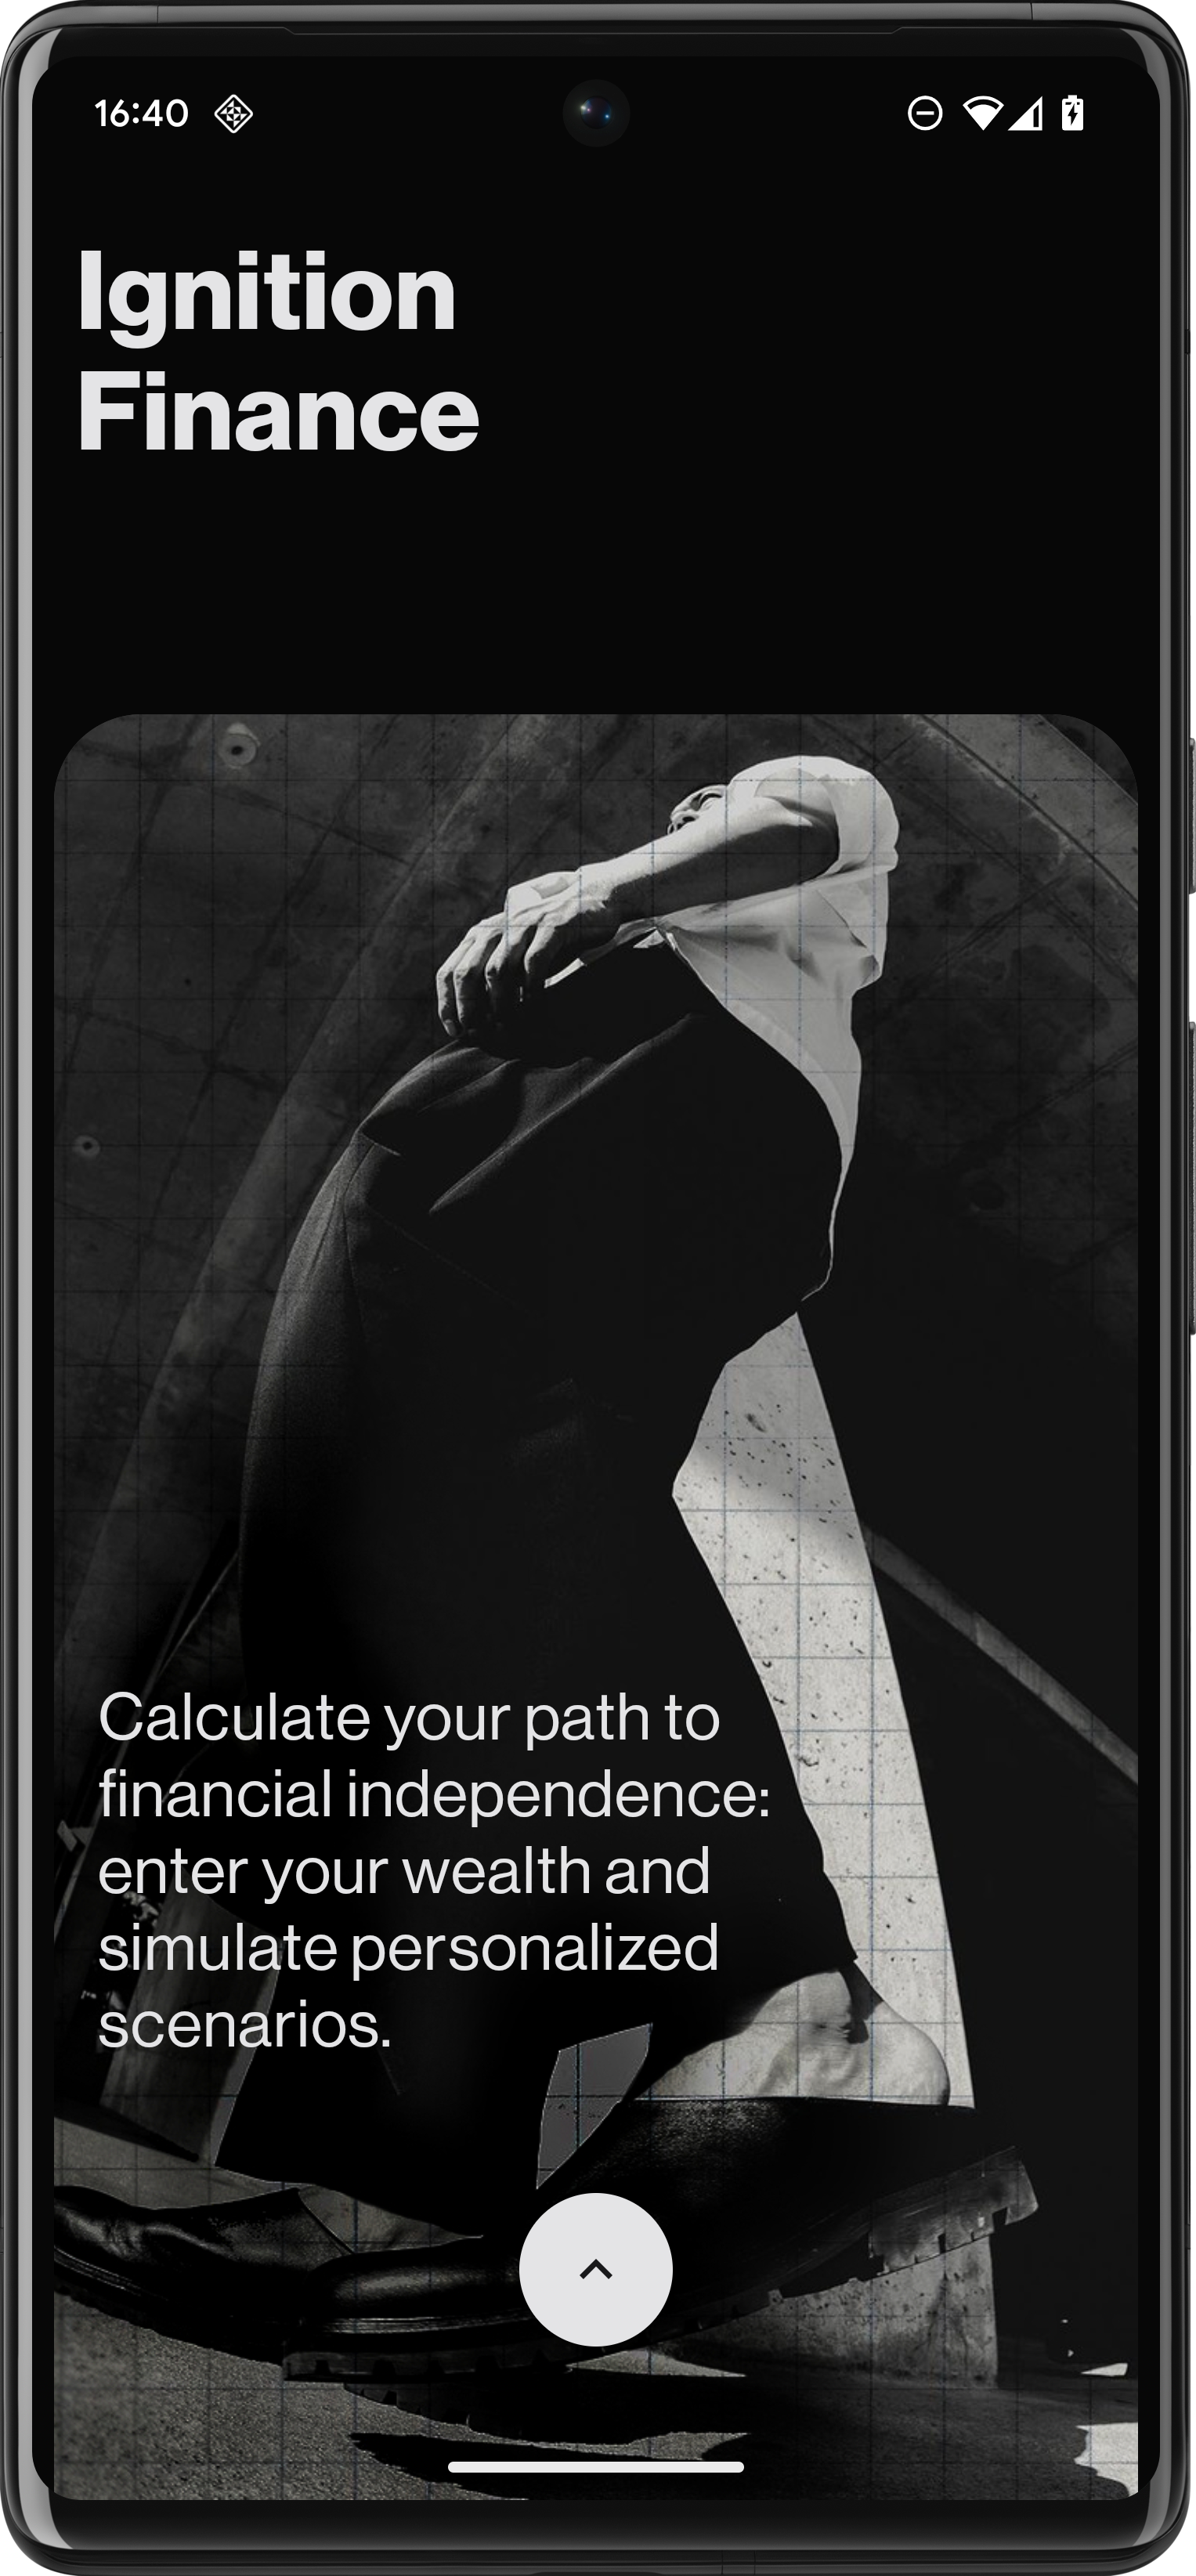
\includegraphics[width=\textwidth]{foto/intro_screen}
        \label{fig:intro_screen}
    \end{minipage}
    \hfill
    \begin{minipage}{0.24\textwidth}
        \centering
        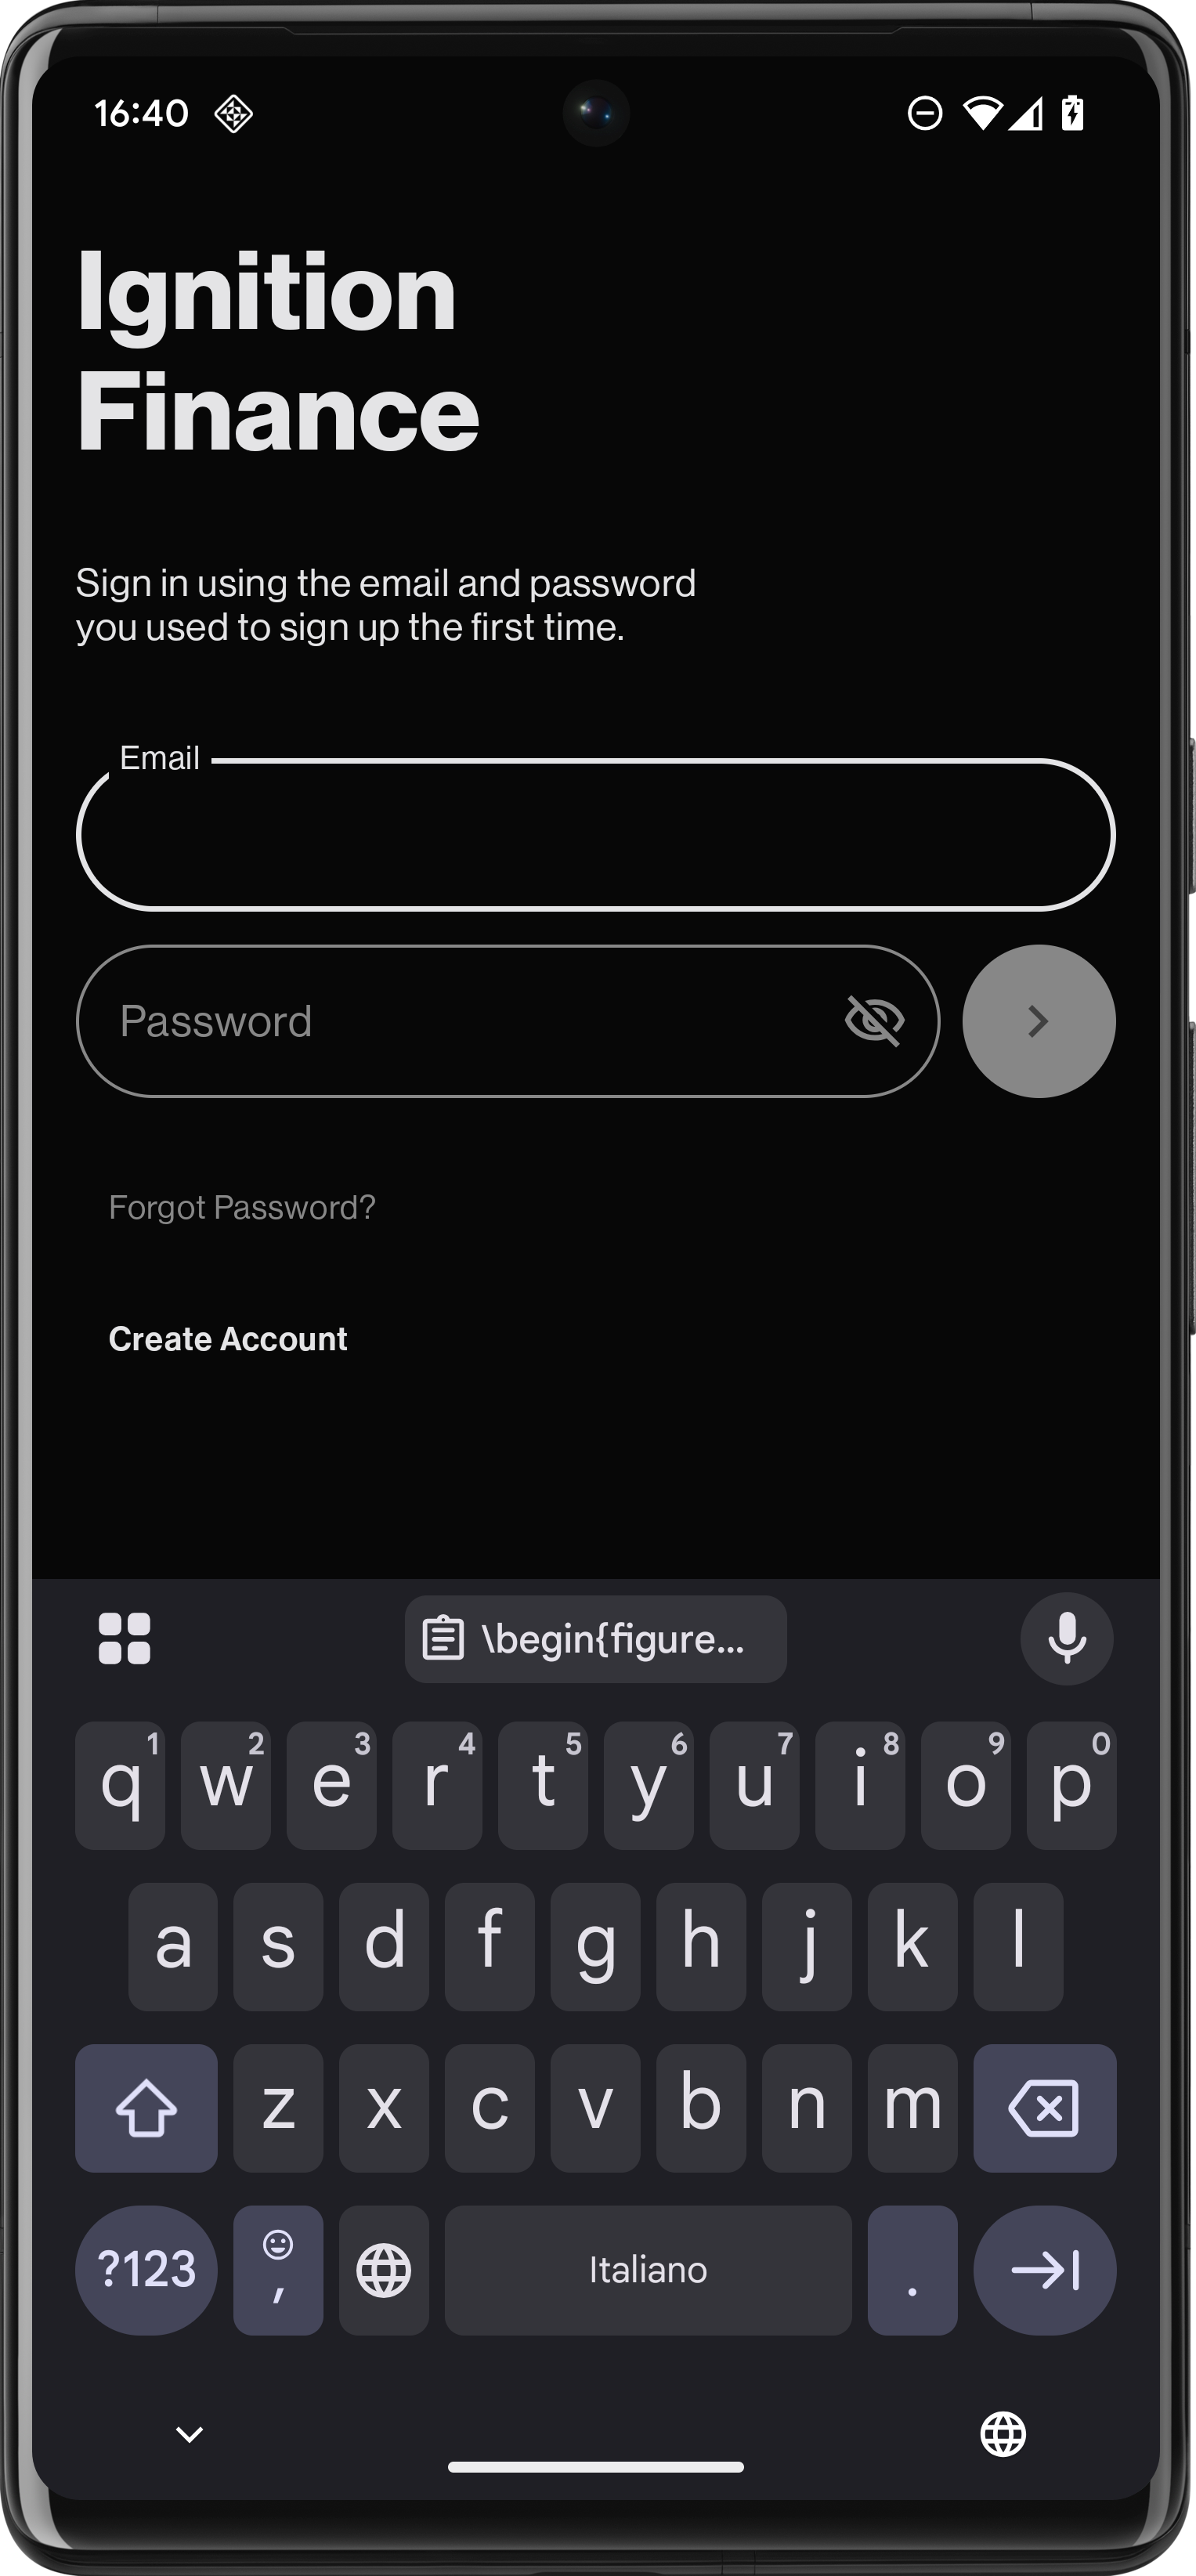
\includegraphics[width=\textwidth]{foto/login}
        \label{fig:login}
    \end{minipage}
    \hfill
    \begin{minipage}{0.24\textwidth}
        \centering
        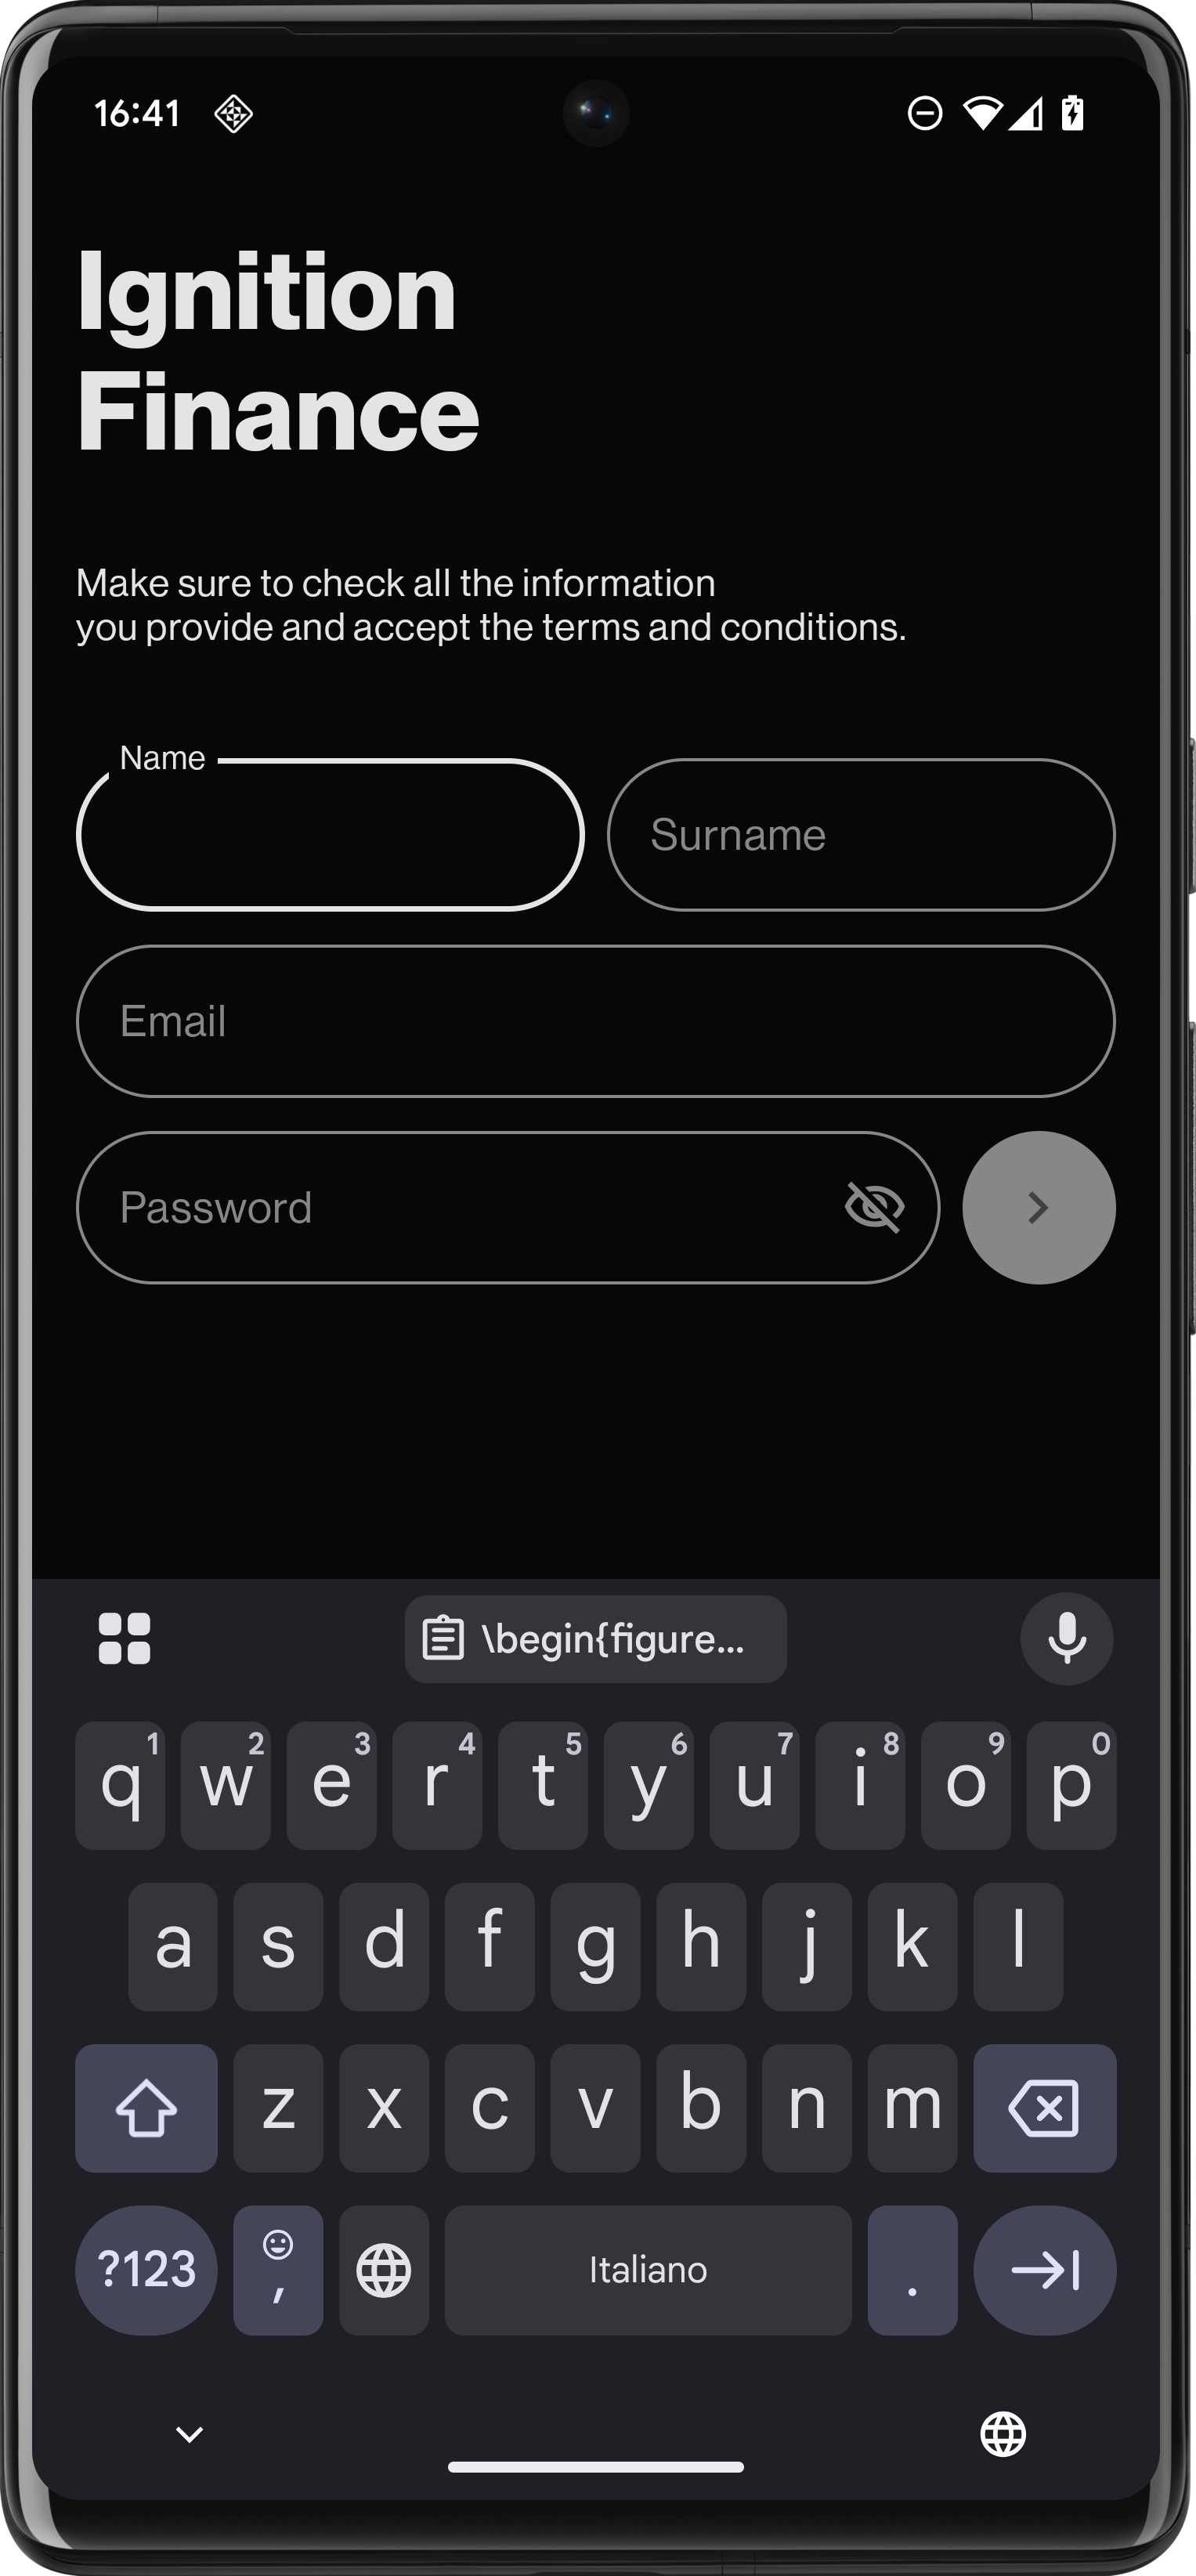
\includegraphics[width=\textwidth]{foto/signup}
        \label{fig:signup}
    \end{minipage}
    \hfill
    \begin{minipage}{0.24\textwidth}
        \centering
        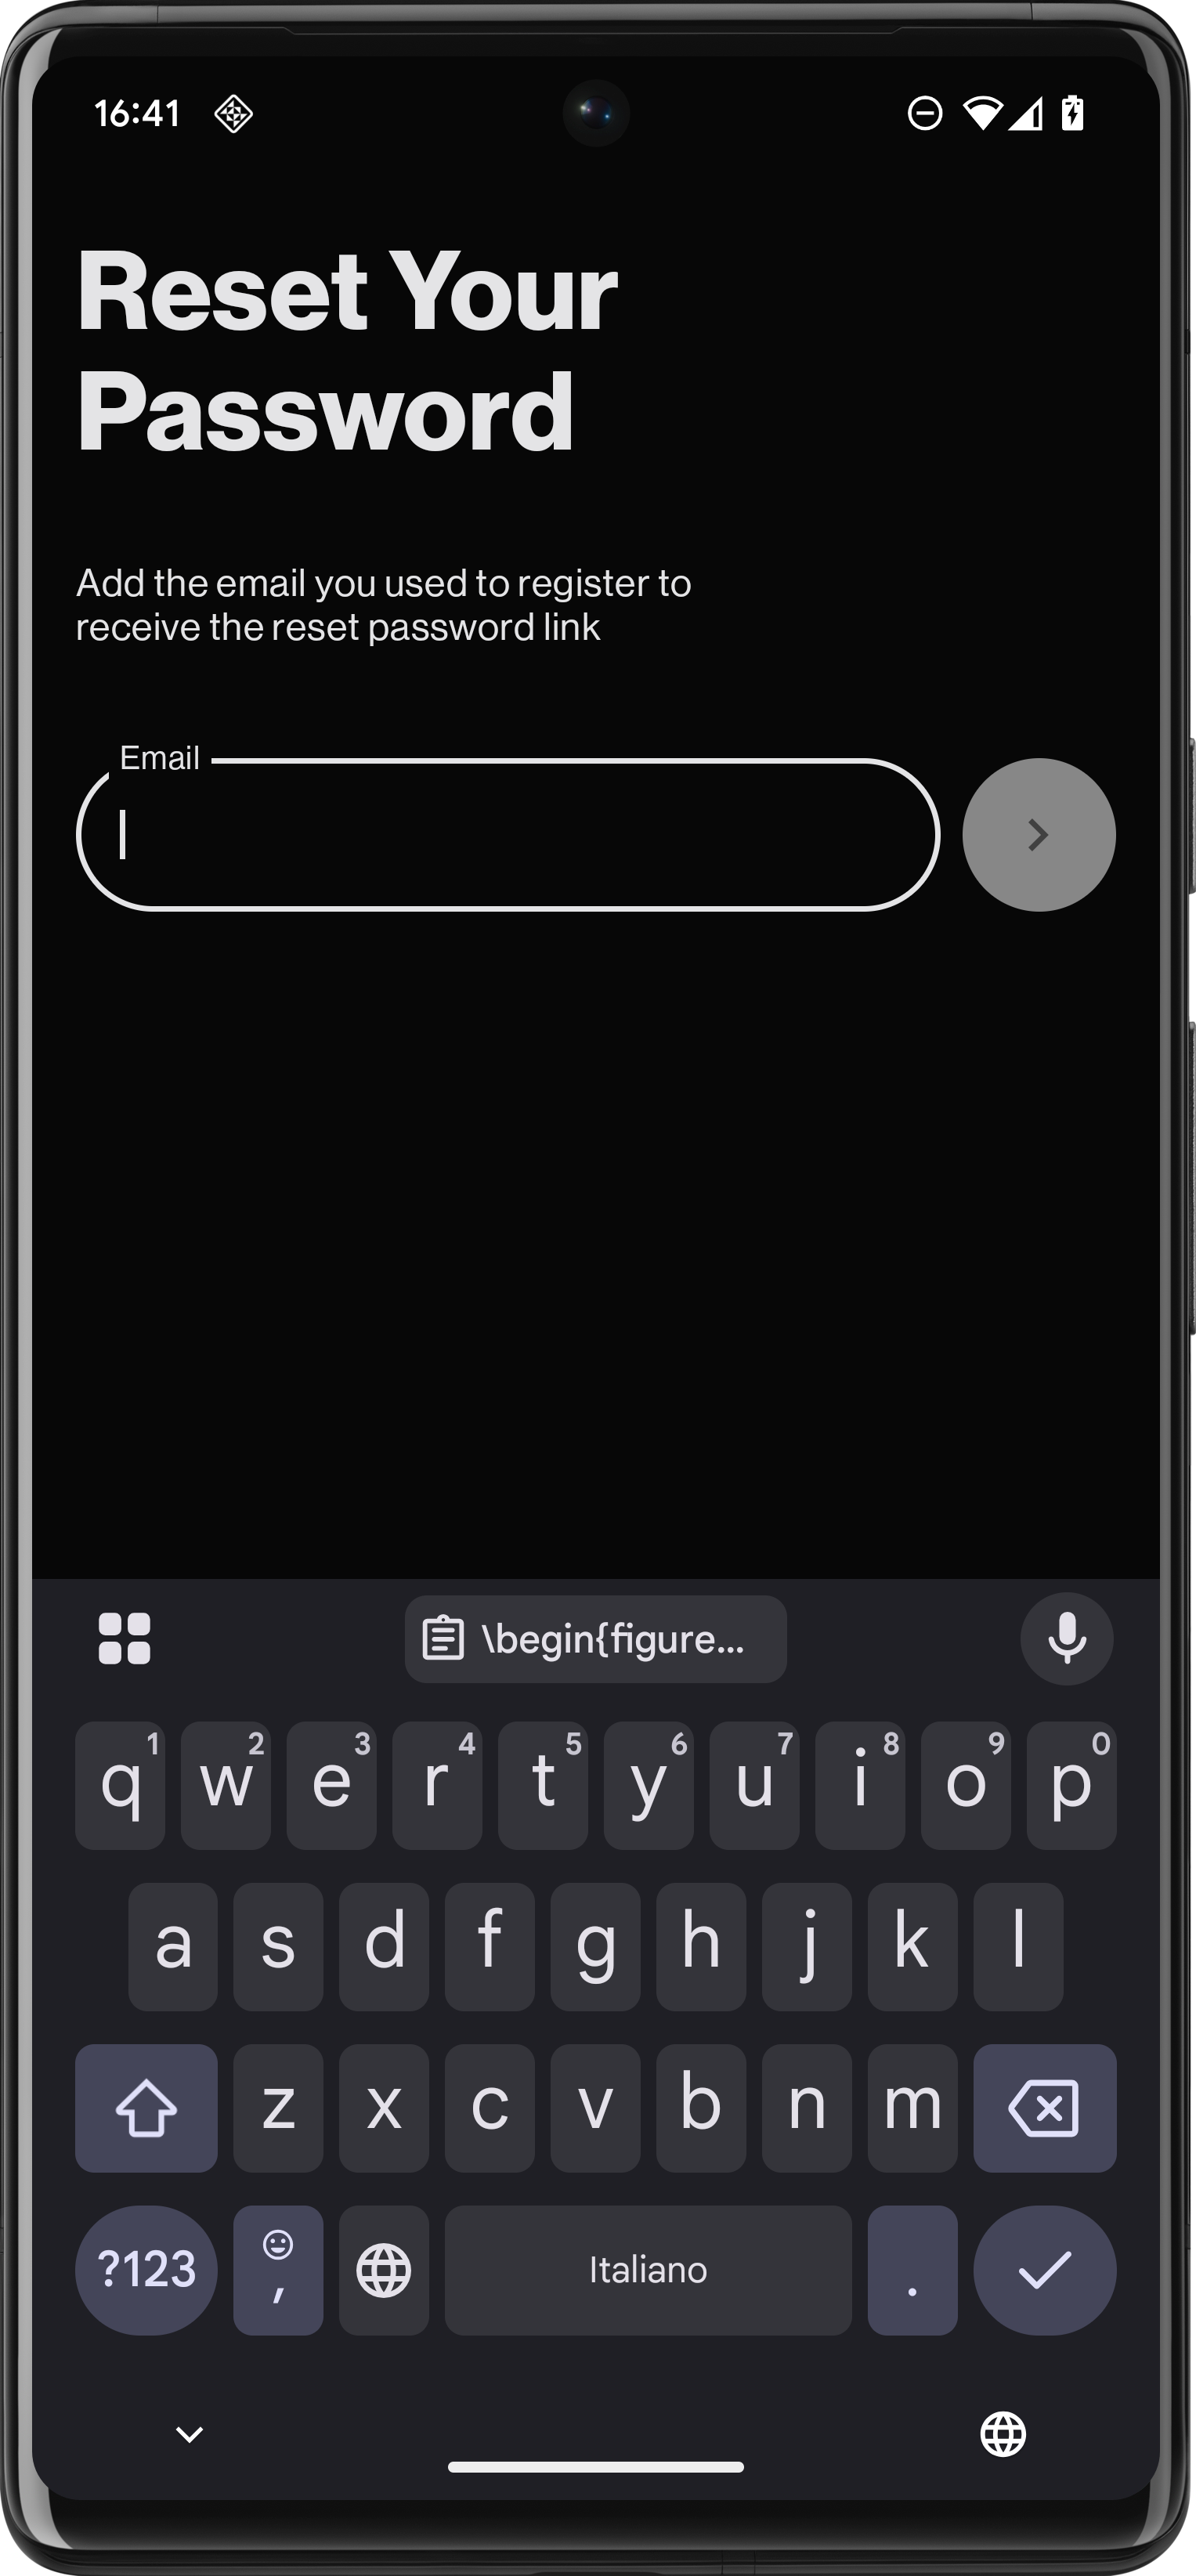
\includegraphics[width=\textwidth]{foto/forgot_password}
        \label{fig:forgot_password}
    \end{minipage}
\end{figure}

\begin{figure}[H]
    \centering
    \begin{minipage}{0.24\textwidth}
        \centering
        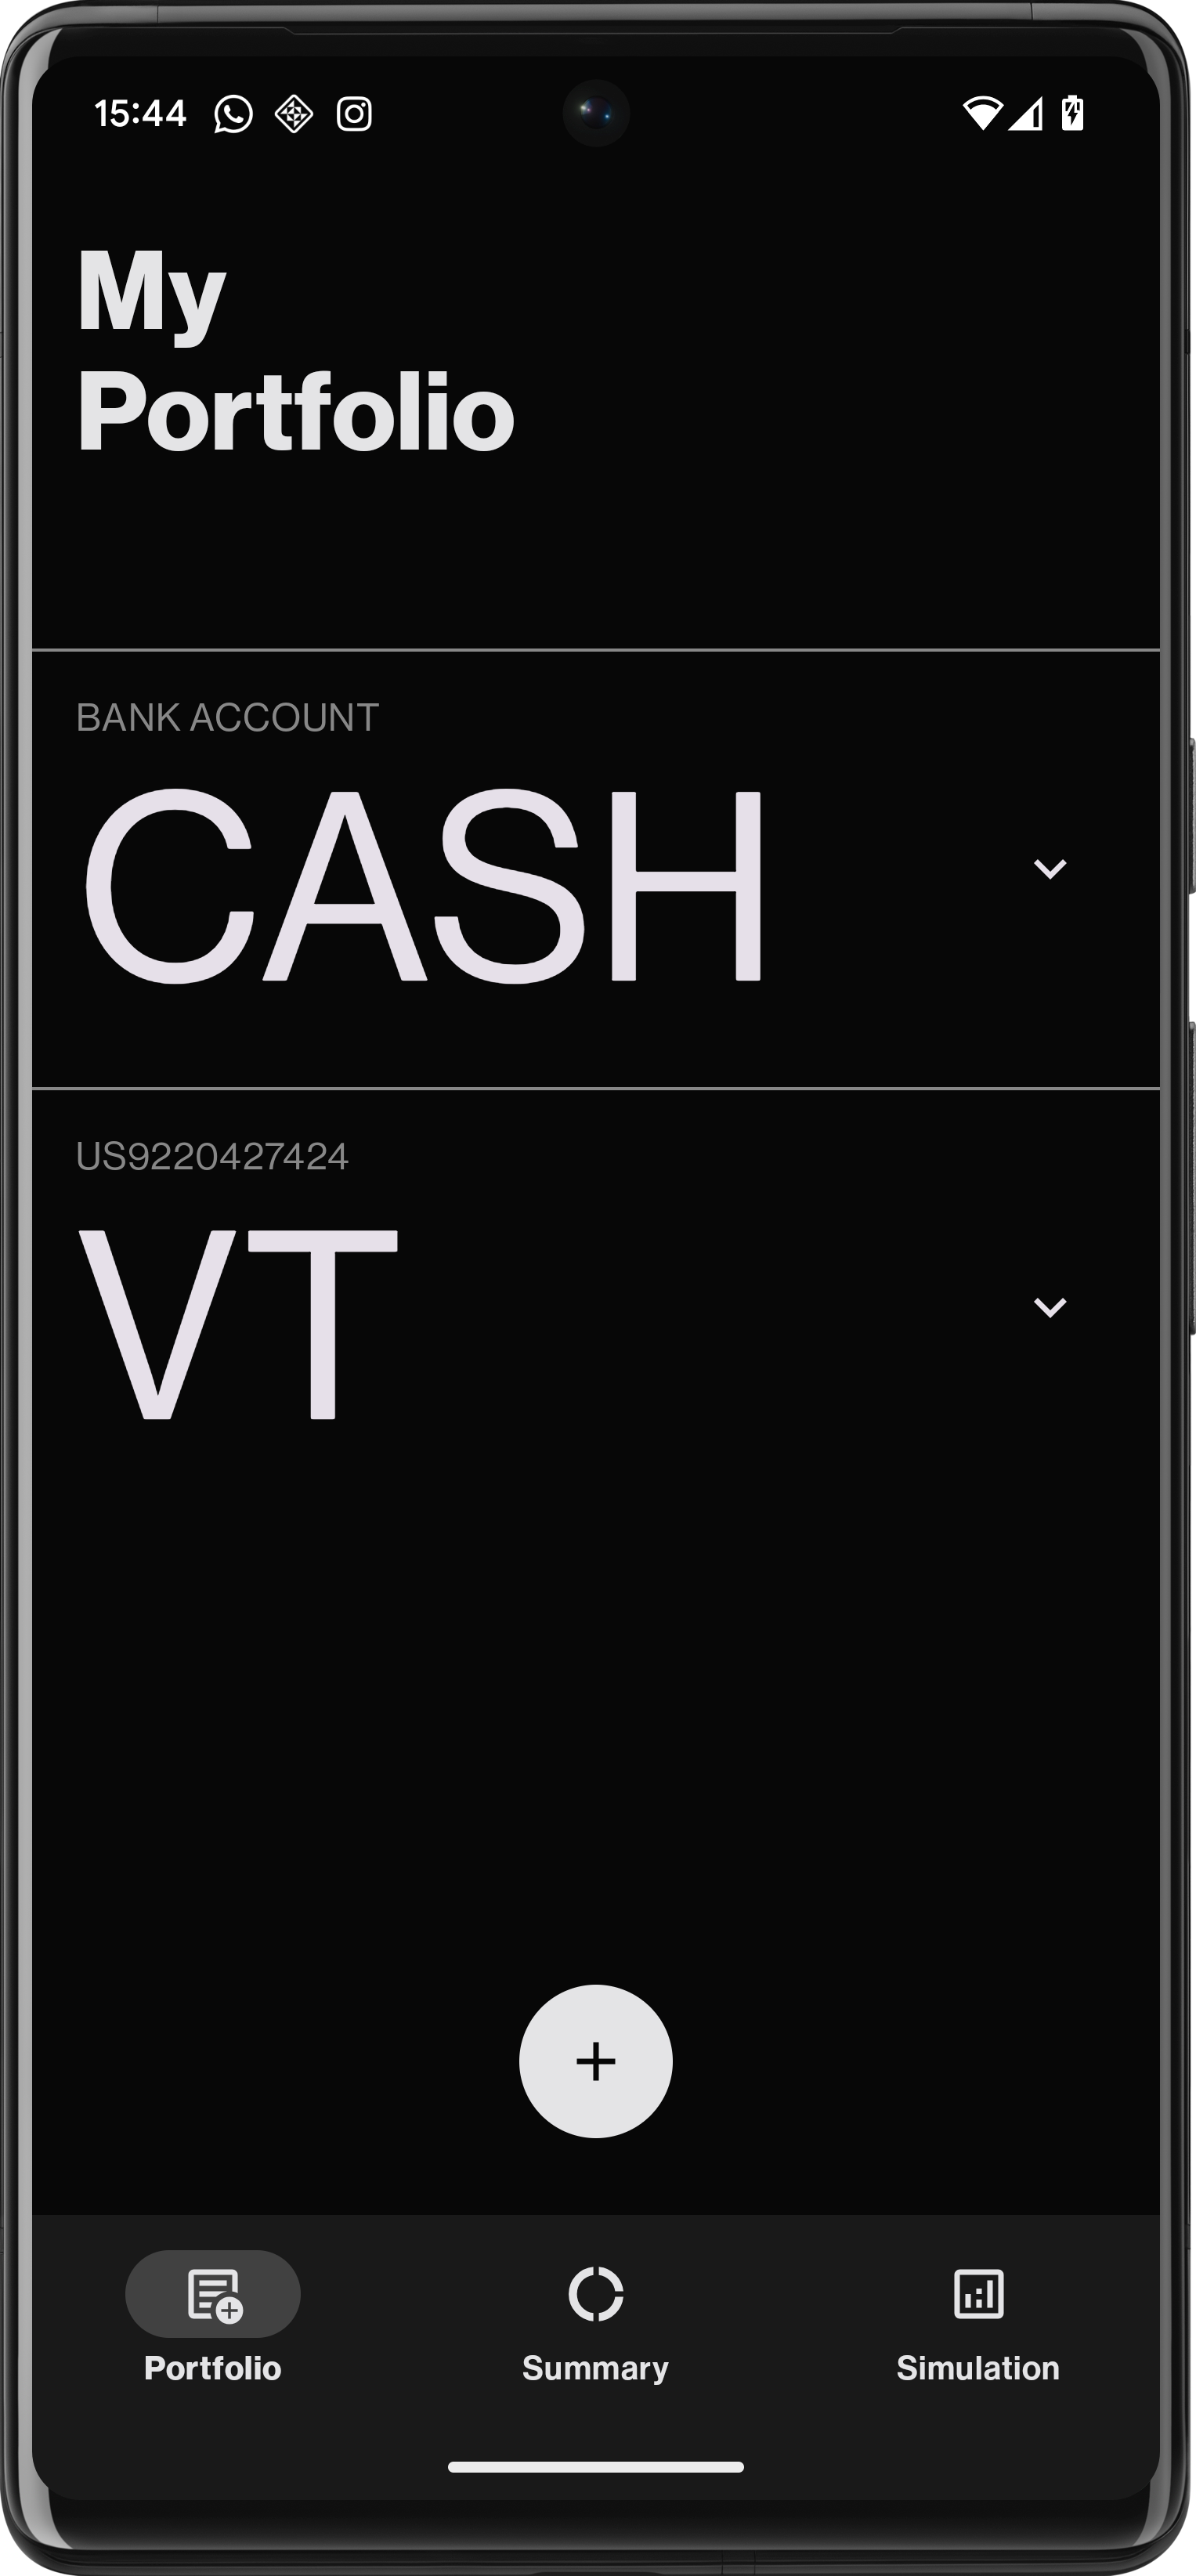
\includegraphics[width=\textwidth]{foto/portfolio_screen}
        \label{fig:portfolio_card}
    \end{minipage}
    \hfill
    \begin{minipage}{0.24\textwidth}
        \centering
        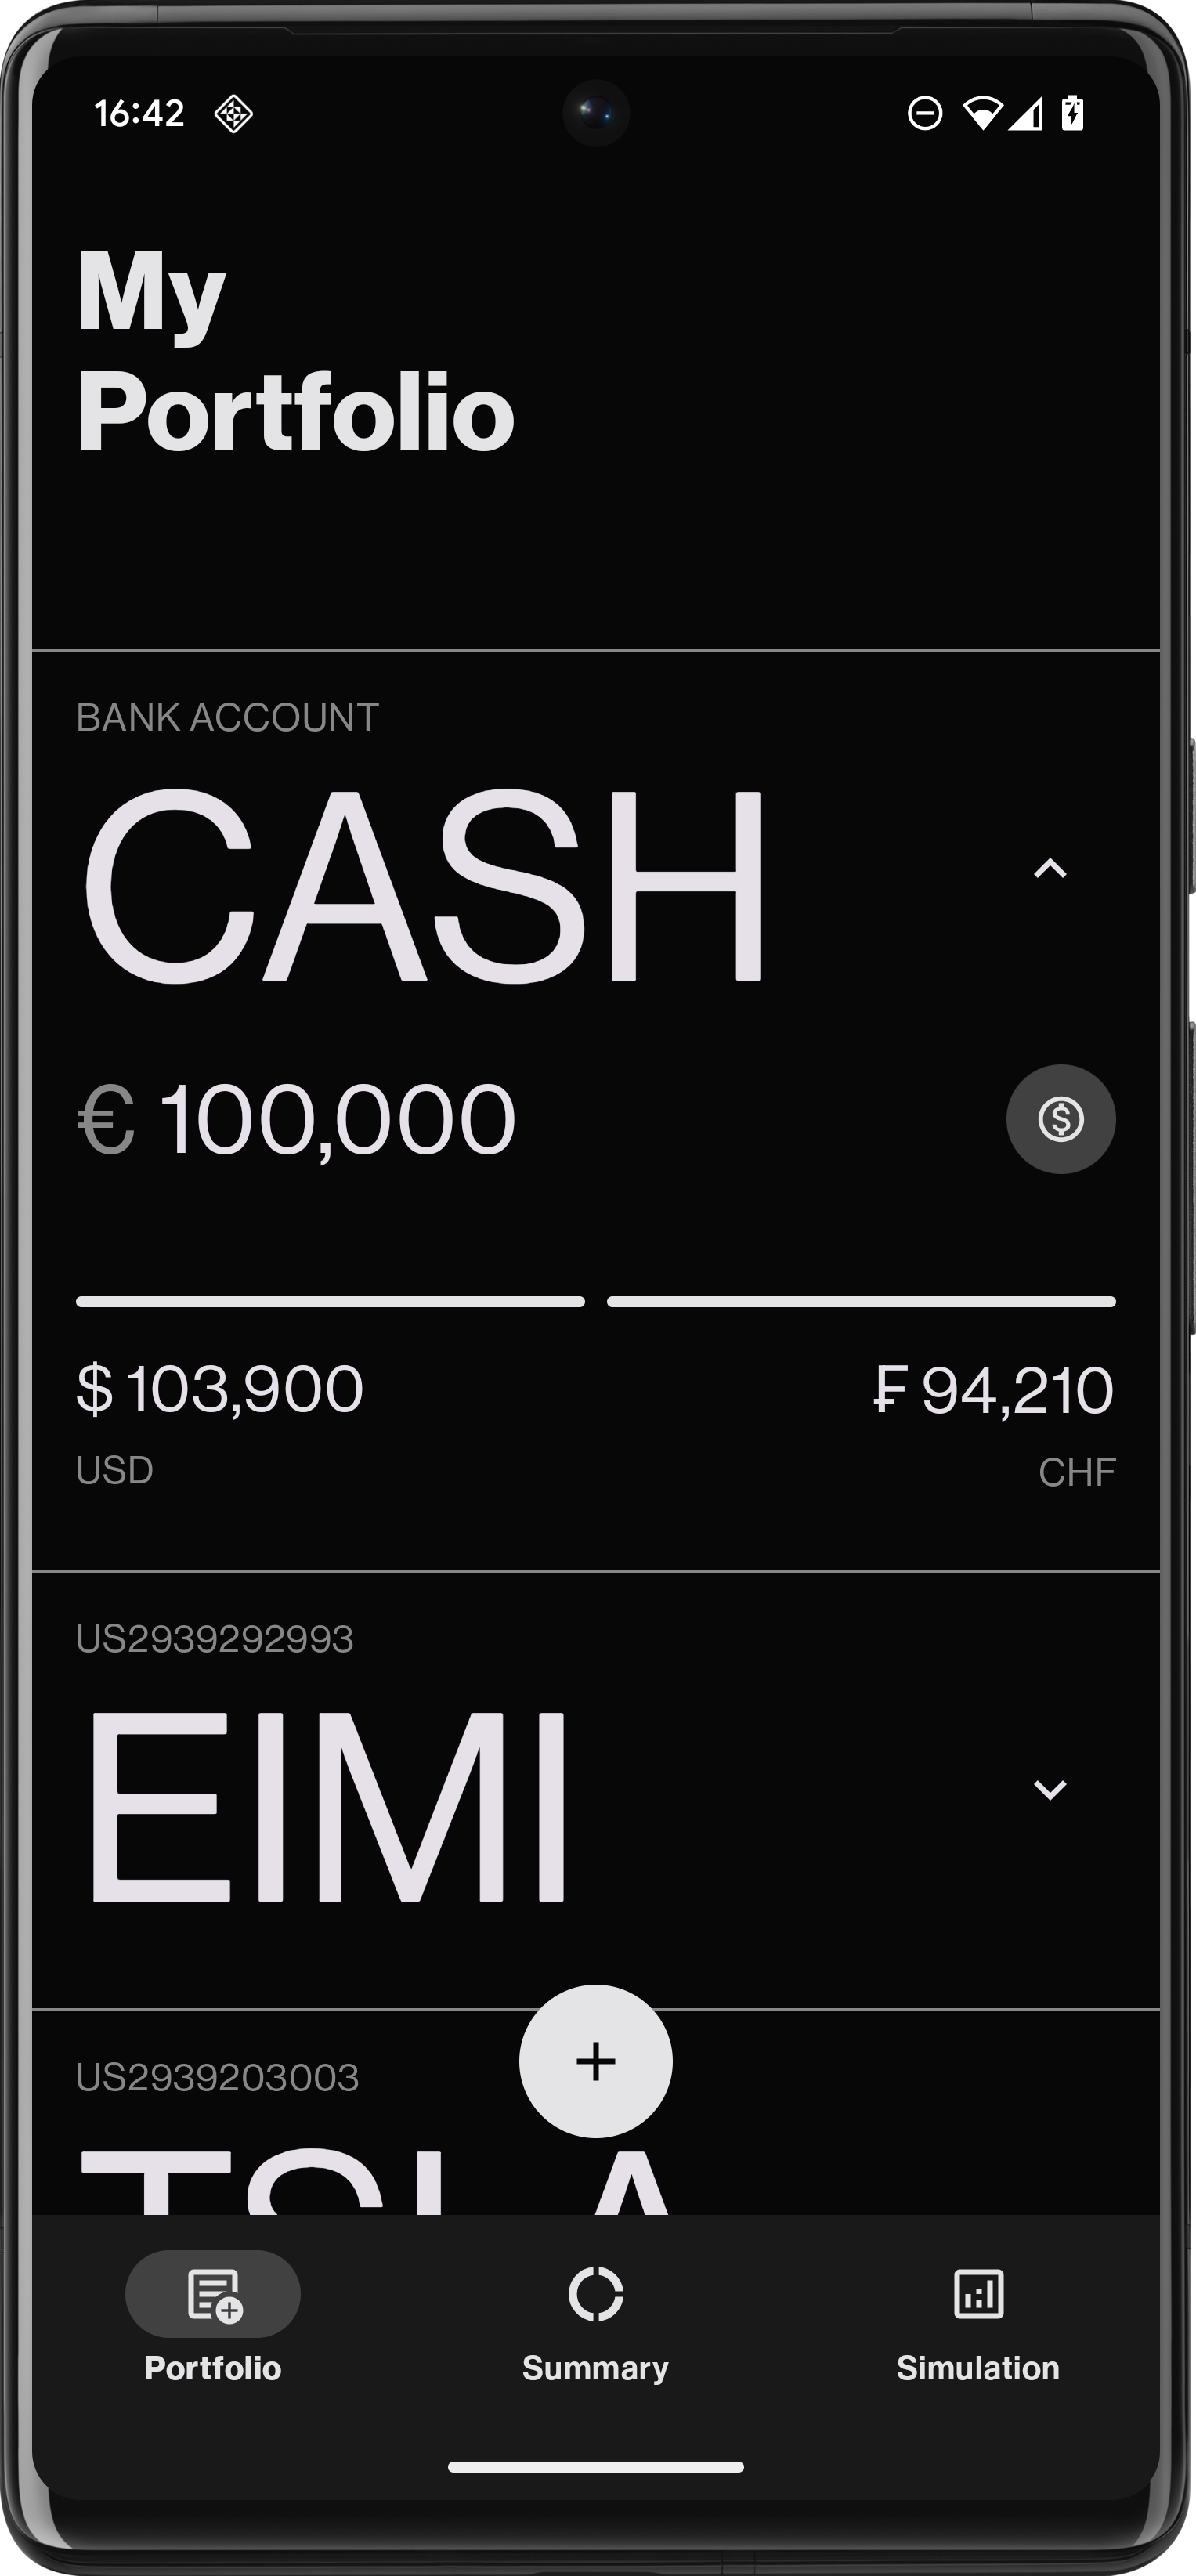
\includegraphics[width=\textwidth]{foto/cash_card}
        \label{fig:cash_card}
    \end{minipage}
    \hfill
    \begin{minipage}{0.24\textwidth}
        \centering
        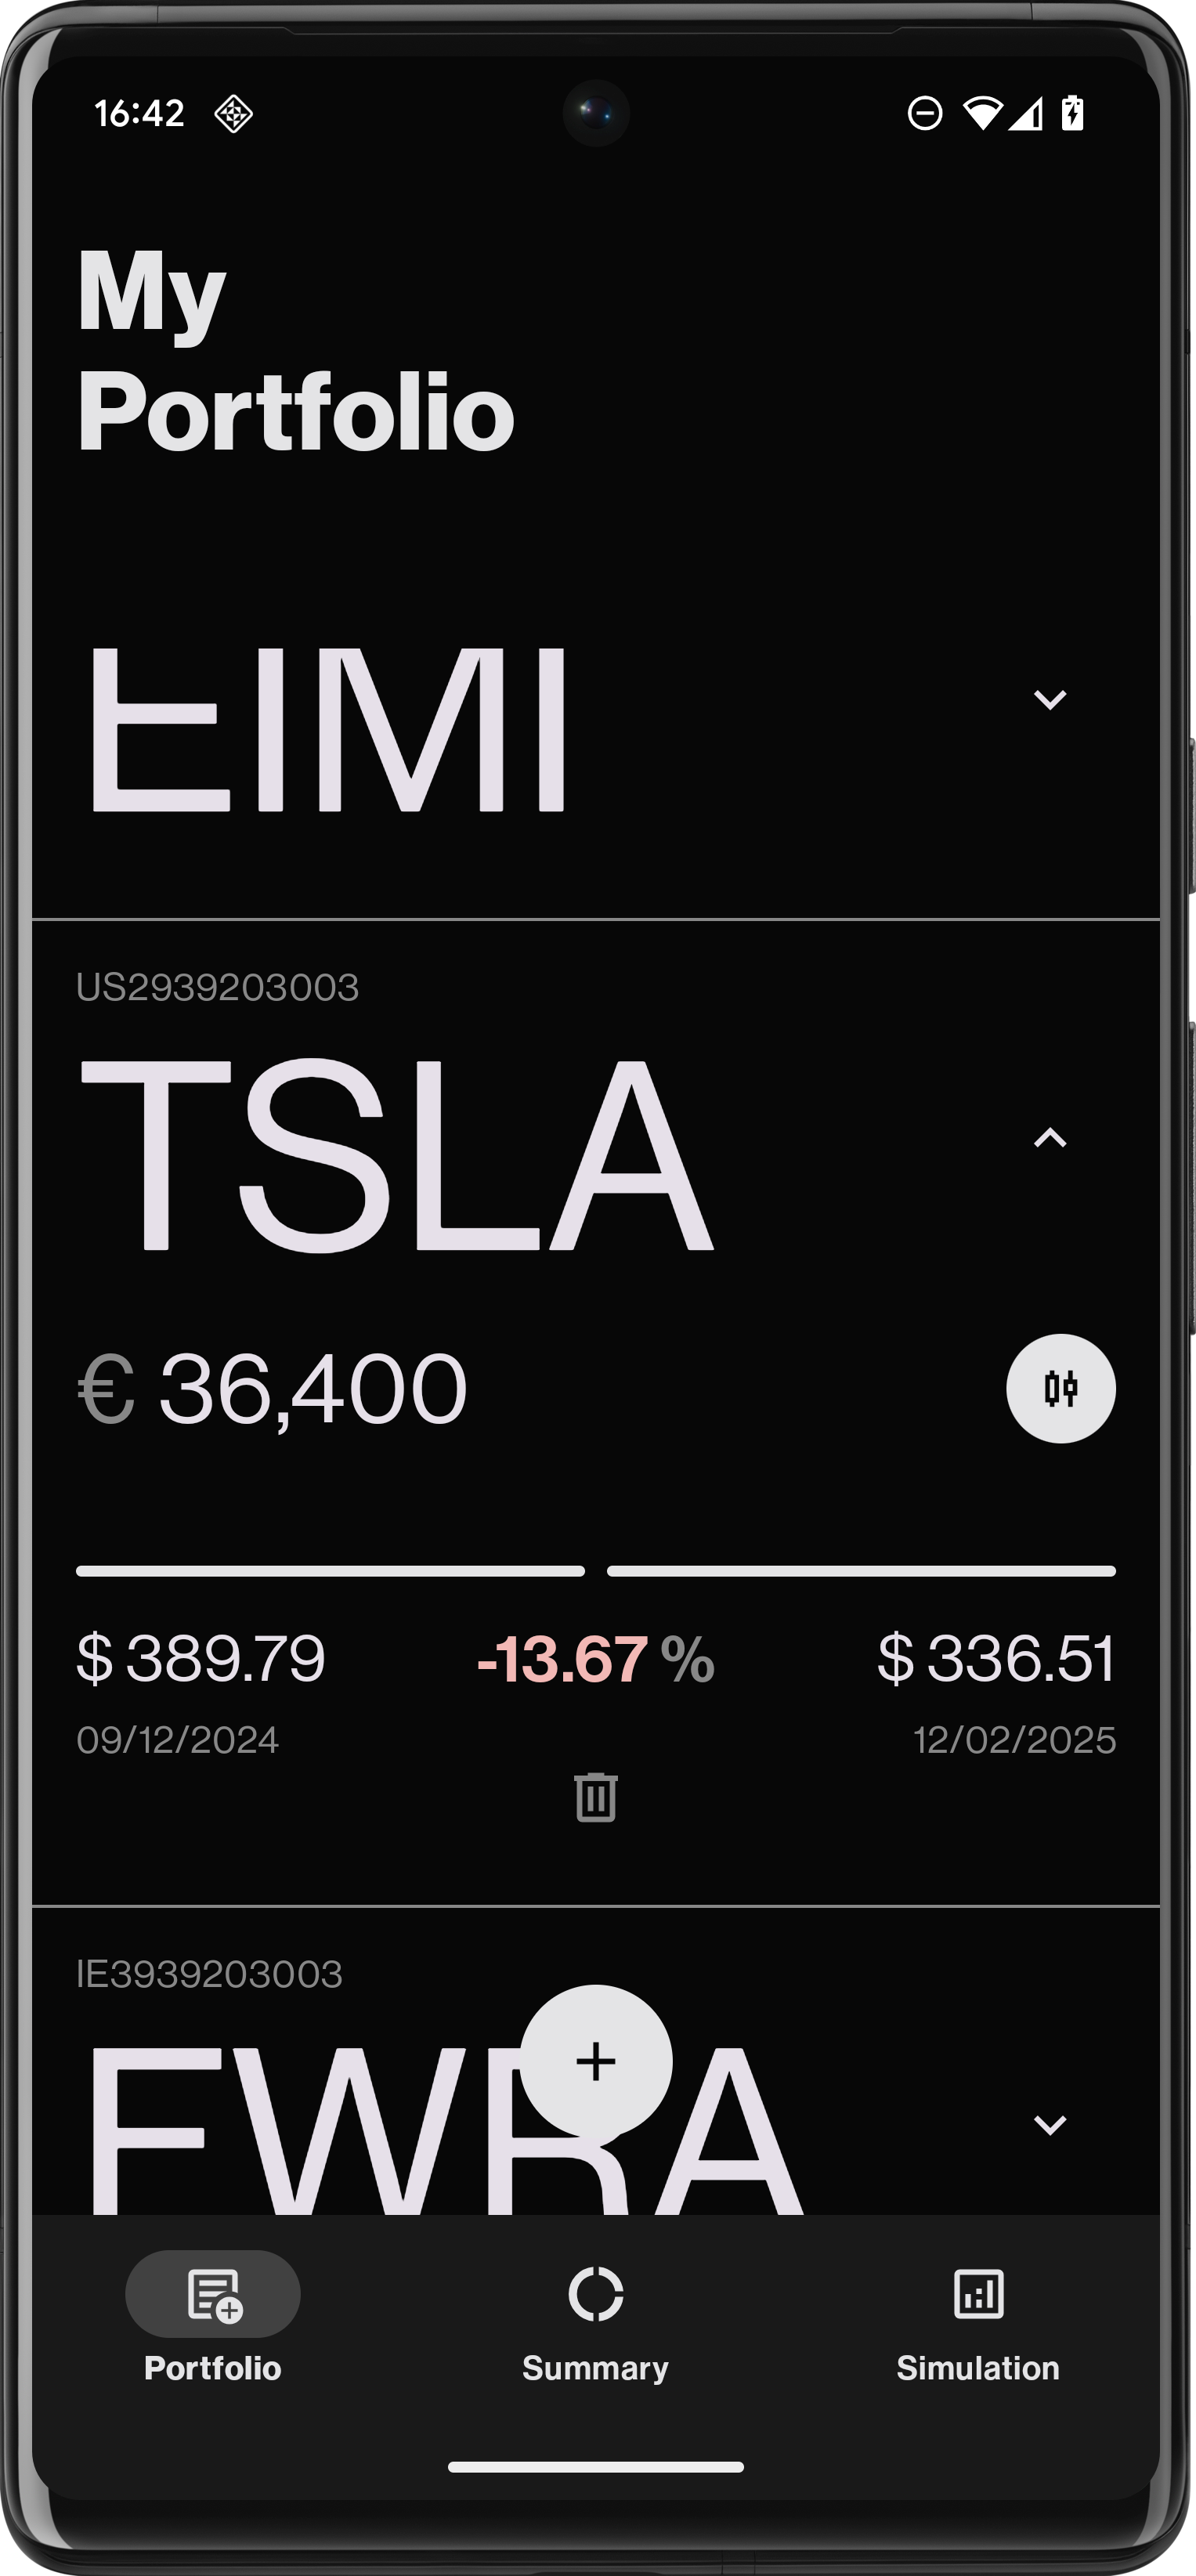
\includegraphics[width=\textwidth]{foto/product_card}
        \label{fig:product_card}
    \end{minipage}
    \hfill
    \begin{minipage}{0.24\textwidth}
        \centering
        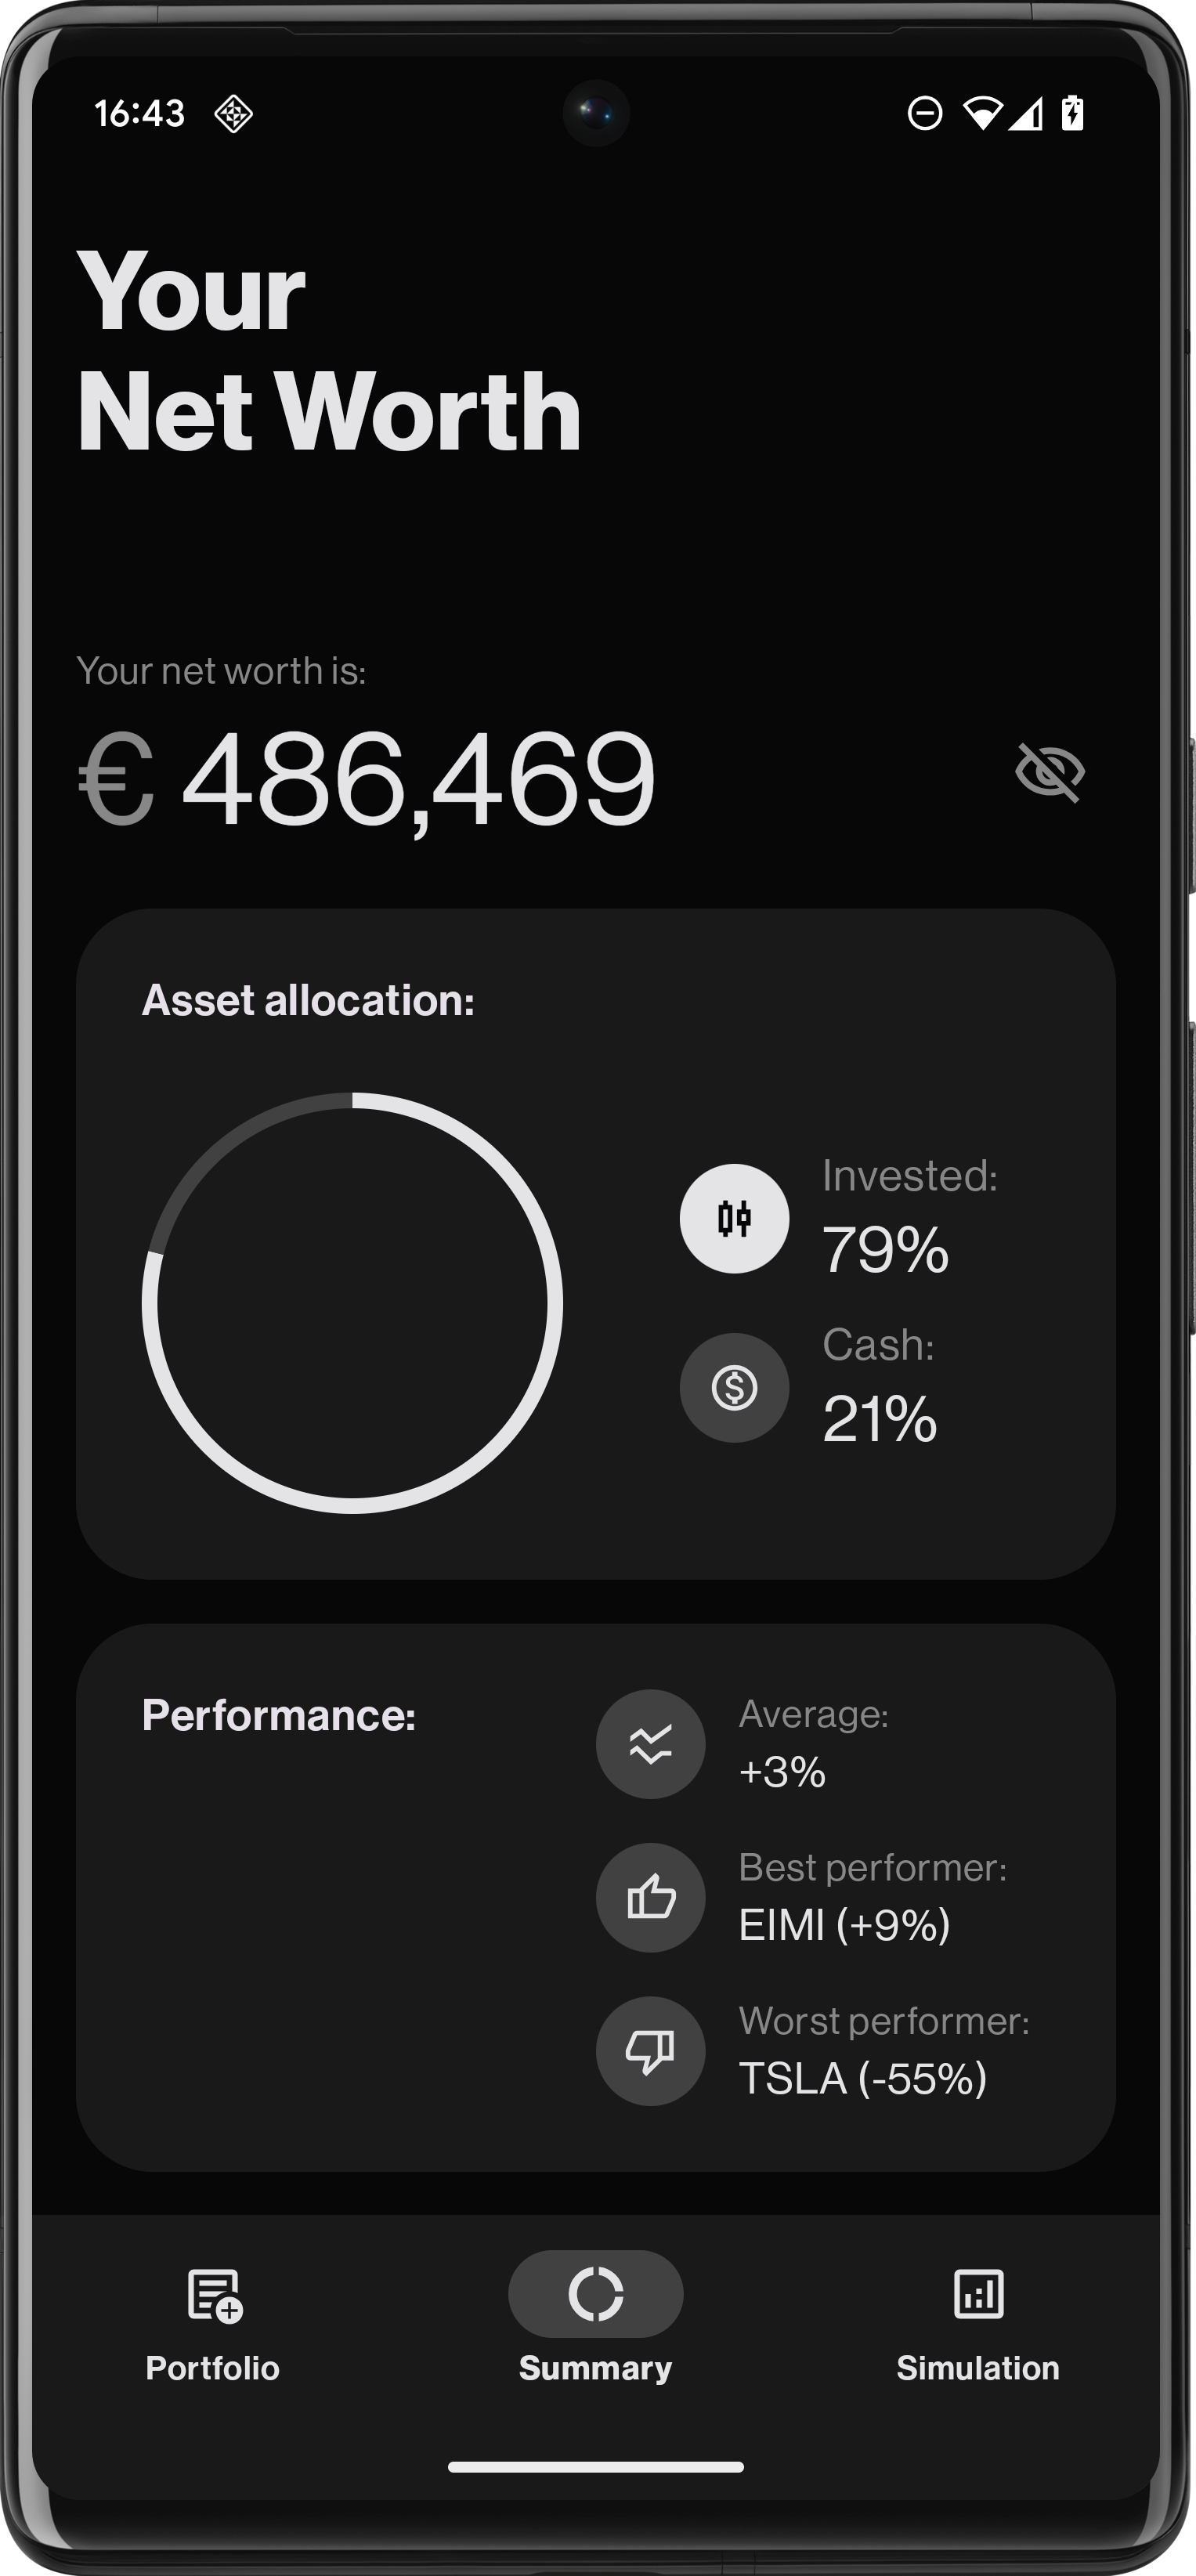
\includegraphics[width=\textwidth]{foto/summary_screen}
        \label{fig:summary_screen}
    \end{minipage}
\end{figure}

\begin{figure}[H]
    \centering
    \begin{minipage}{0.24\textwidth}
        \centering
        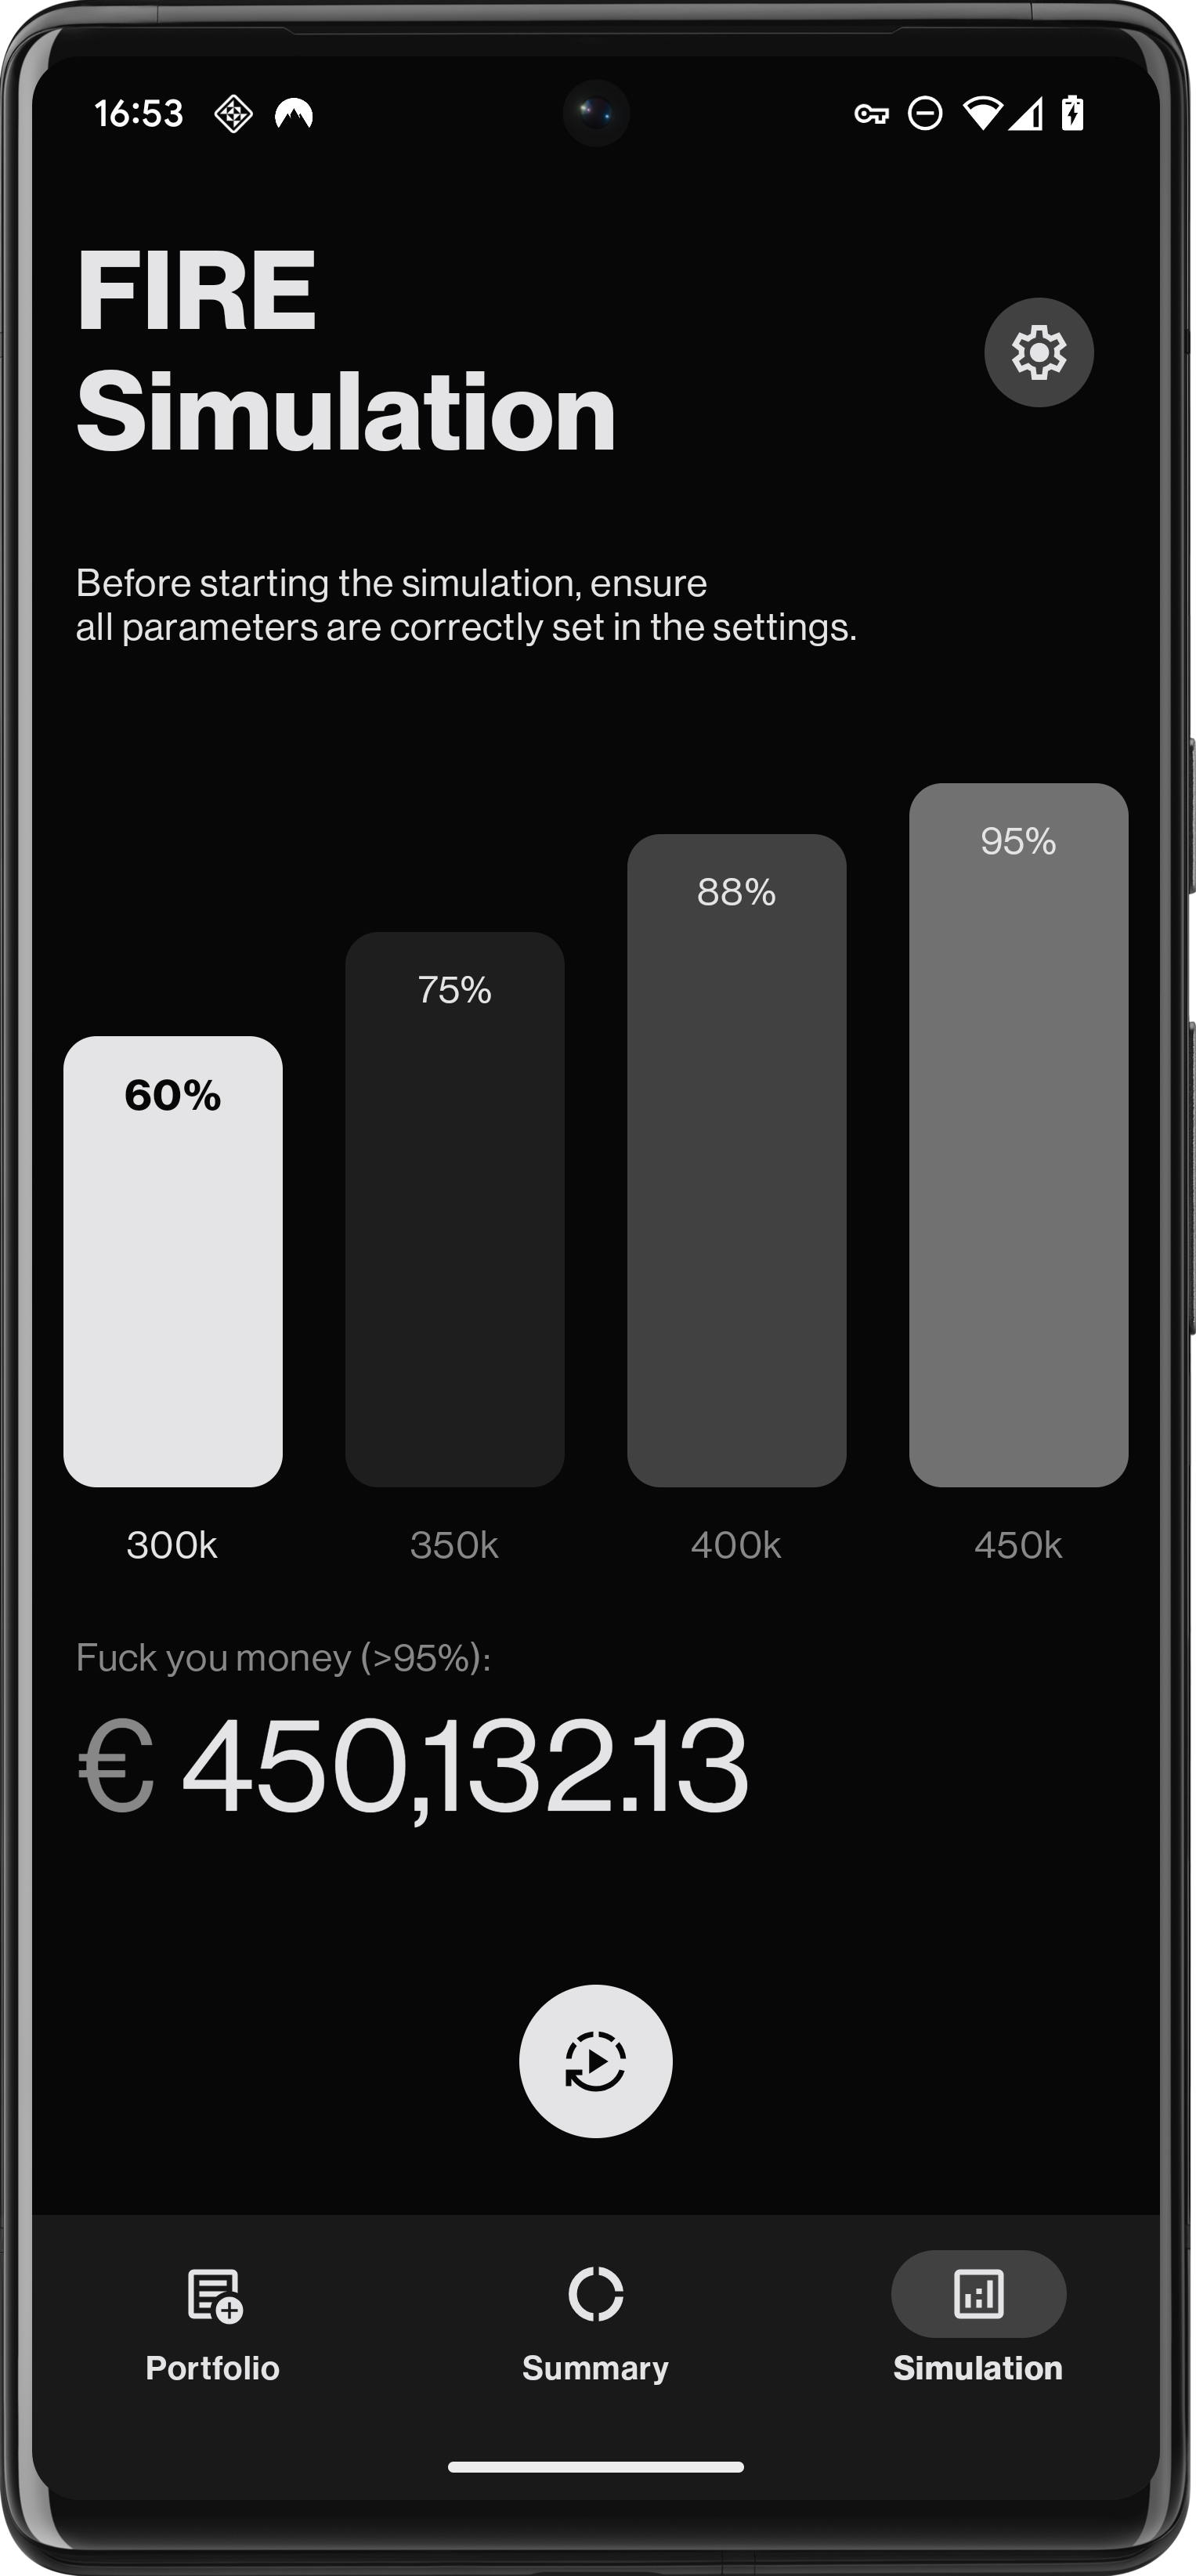
\includegraphics[width=\textwidth]{foto/simulation_screen}
        \label{fig:simulation_screen}
    \end{minipage}
    \hfill
    \begin{minipage}{0.24\textwidth}
        \centering
        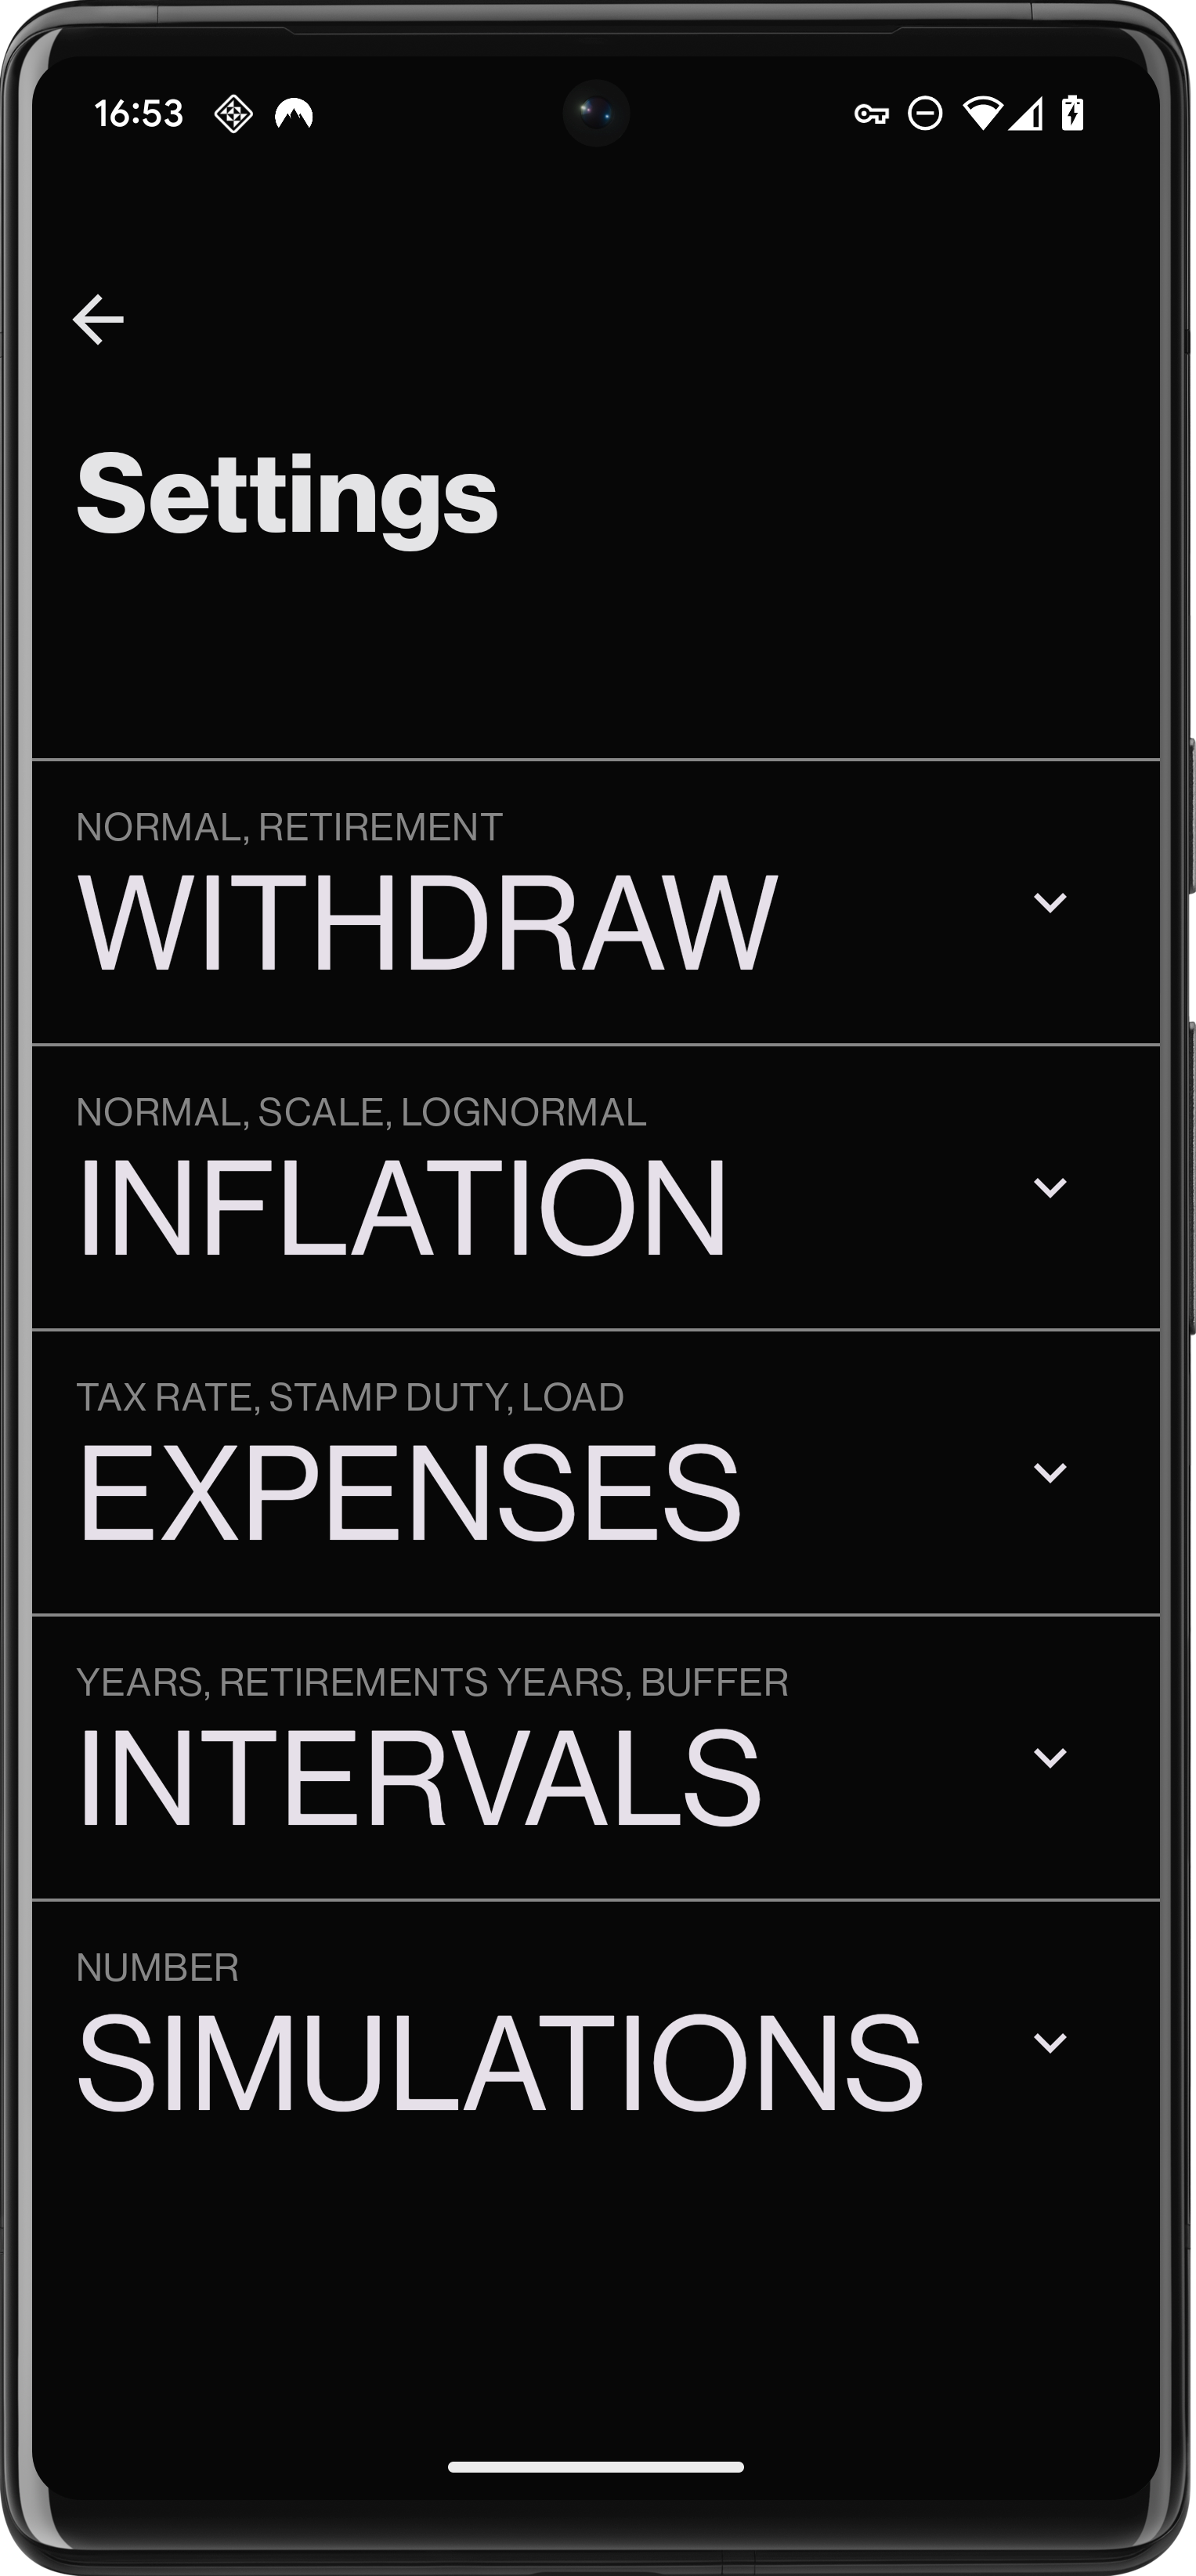
\includegraphics[width=\textwidth]{foto/settings_screen}
        \label{fig:settings_screen}
    \end{minipage}
    \hfill
    \begin{minipage}{0.24\textwidth}
        \centering
        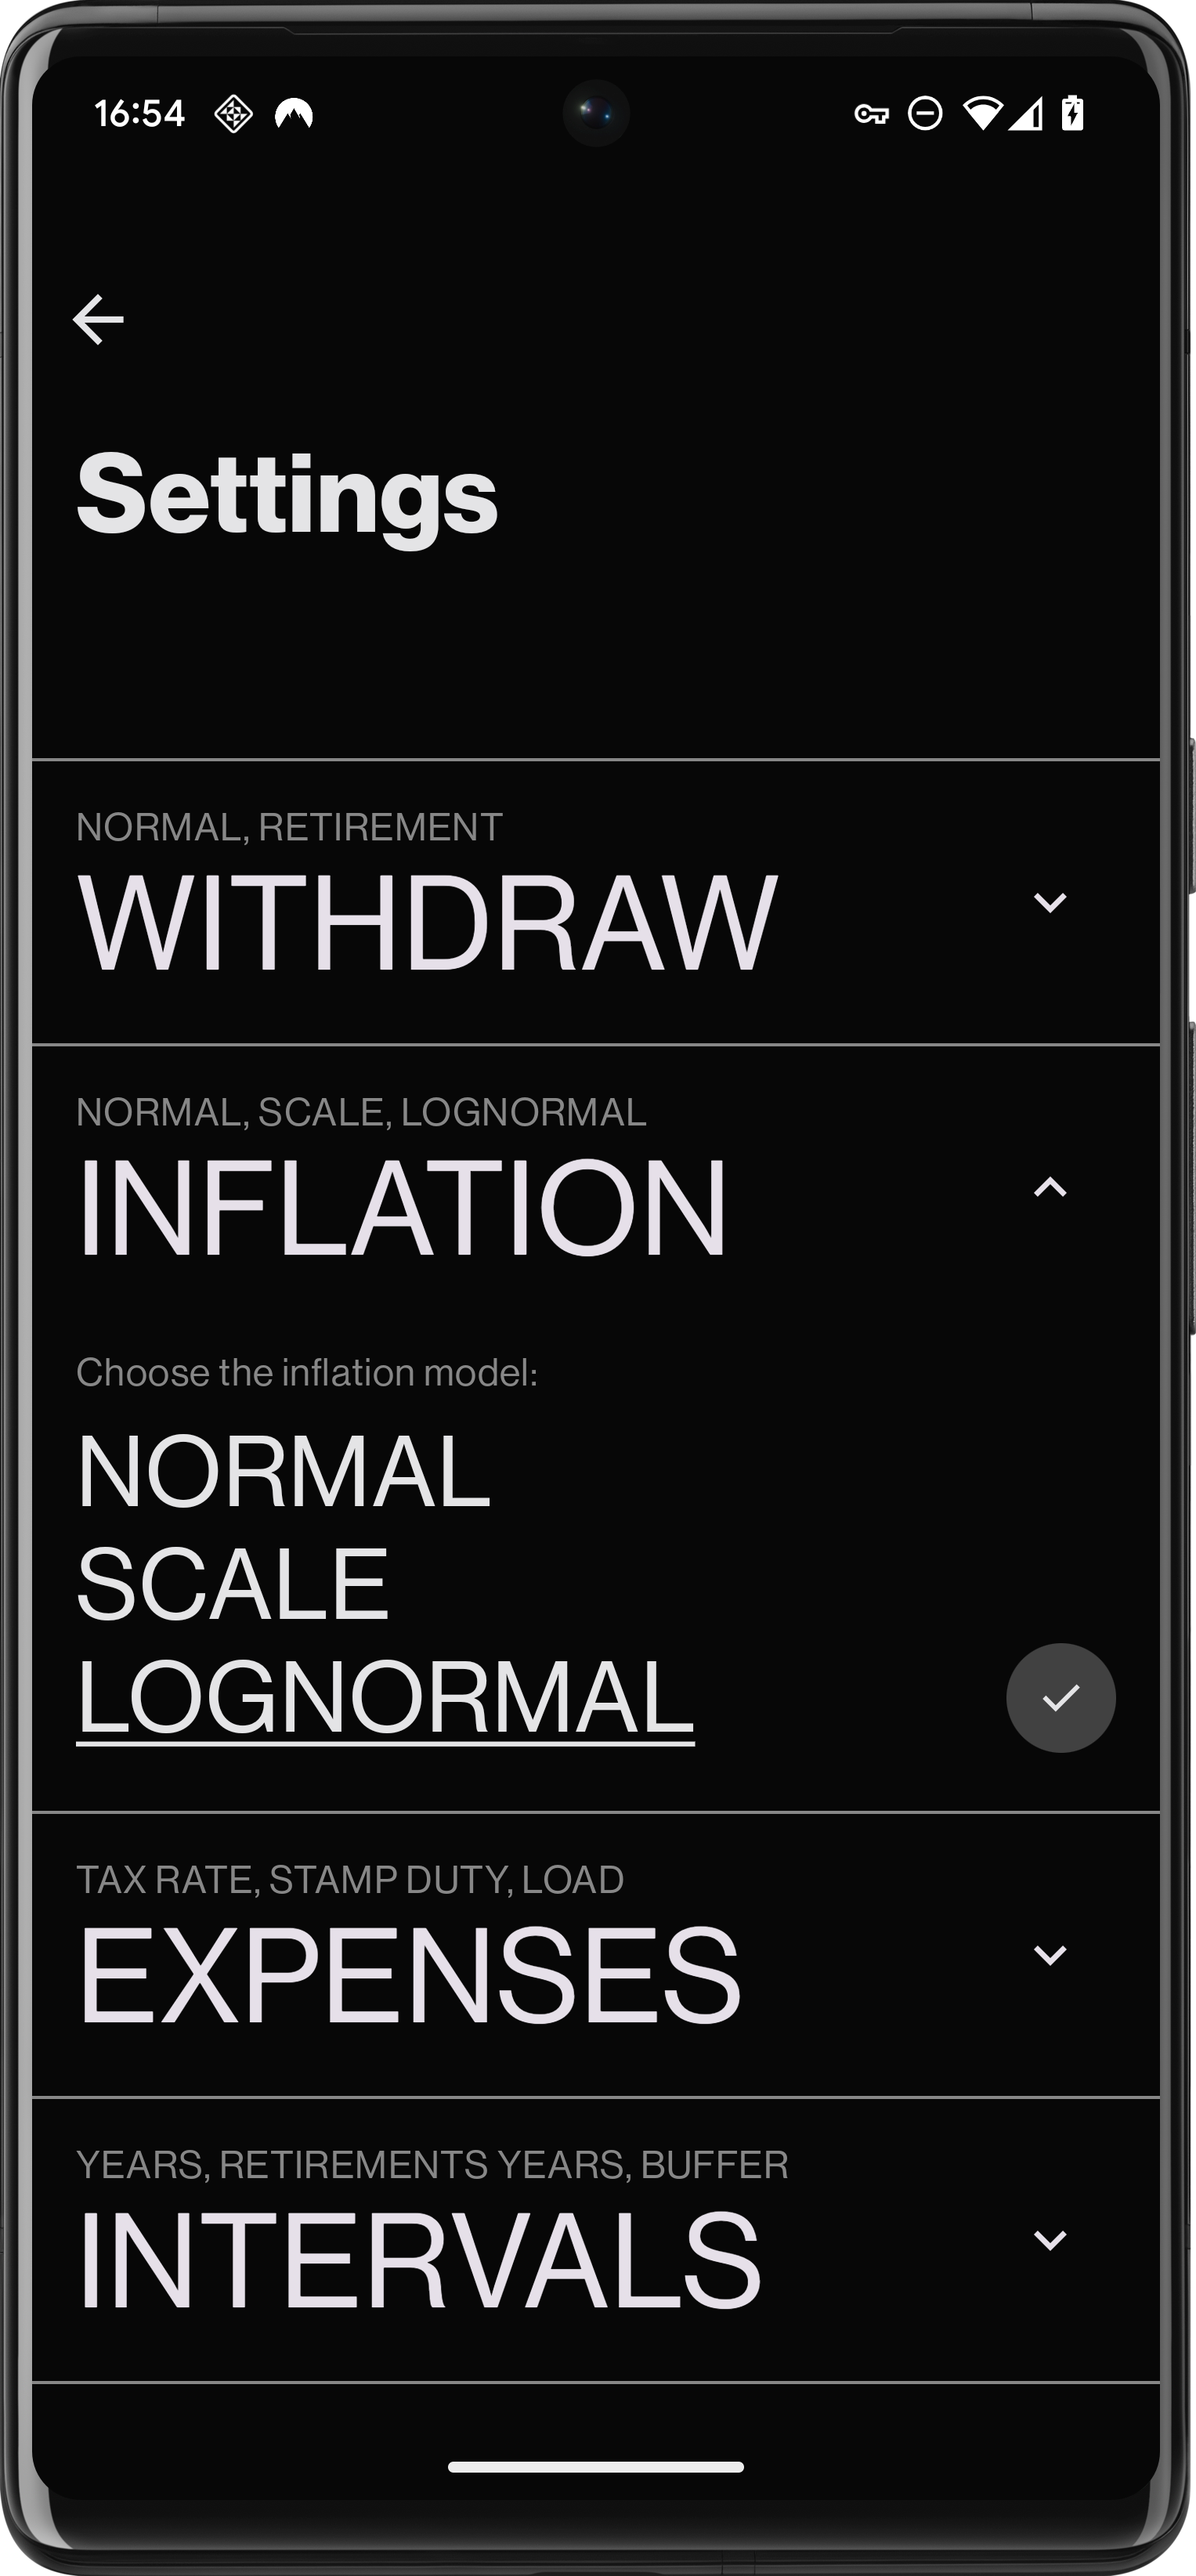
\includegraphics[width=\textwidth]{foto/inflation_card}
        \label{fig:inflation_card}
    \end{minipage}
    \hfill
    \begin{minipage}{0.24\textwidth}
        \centering
        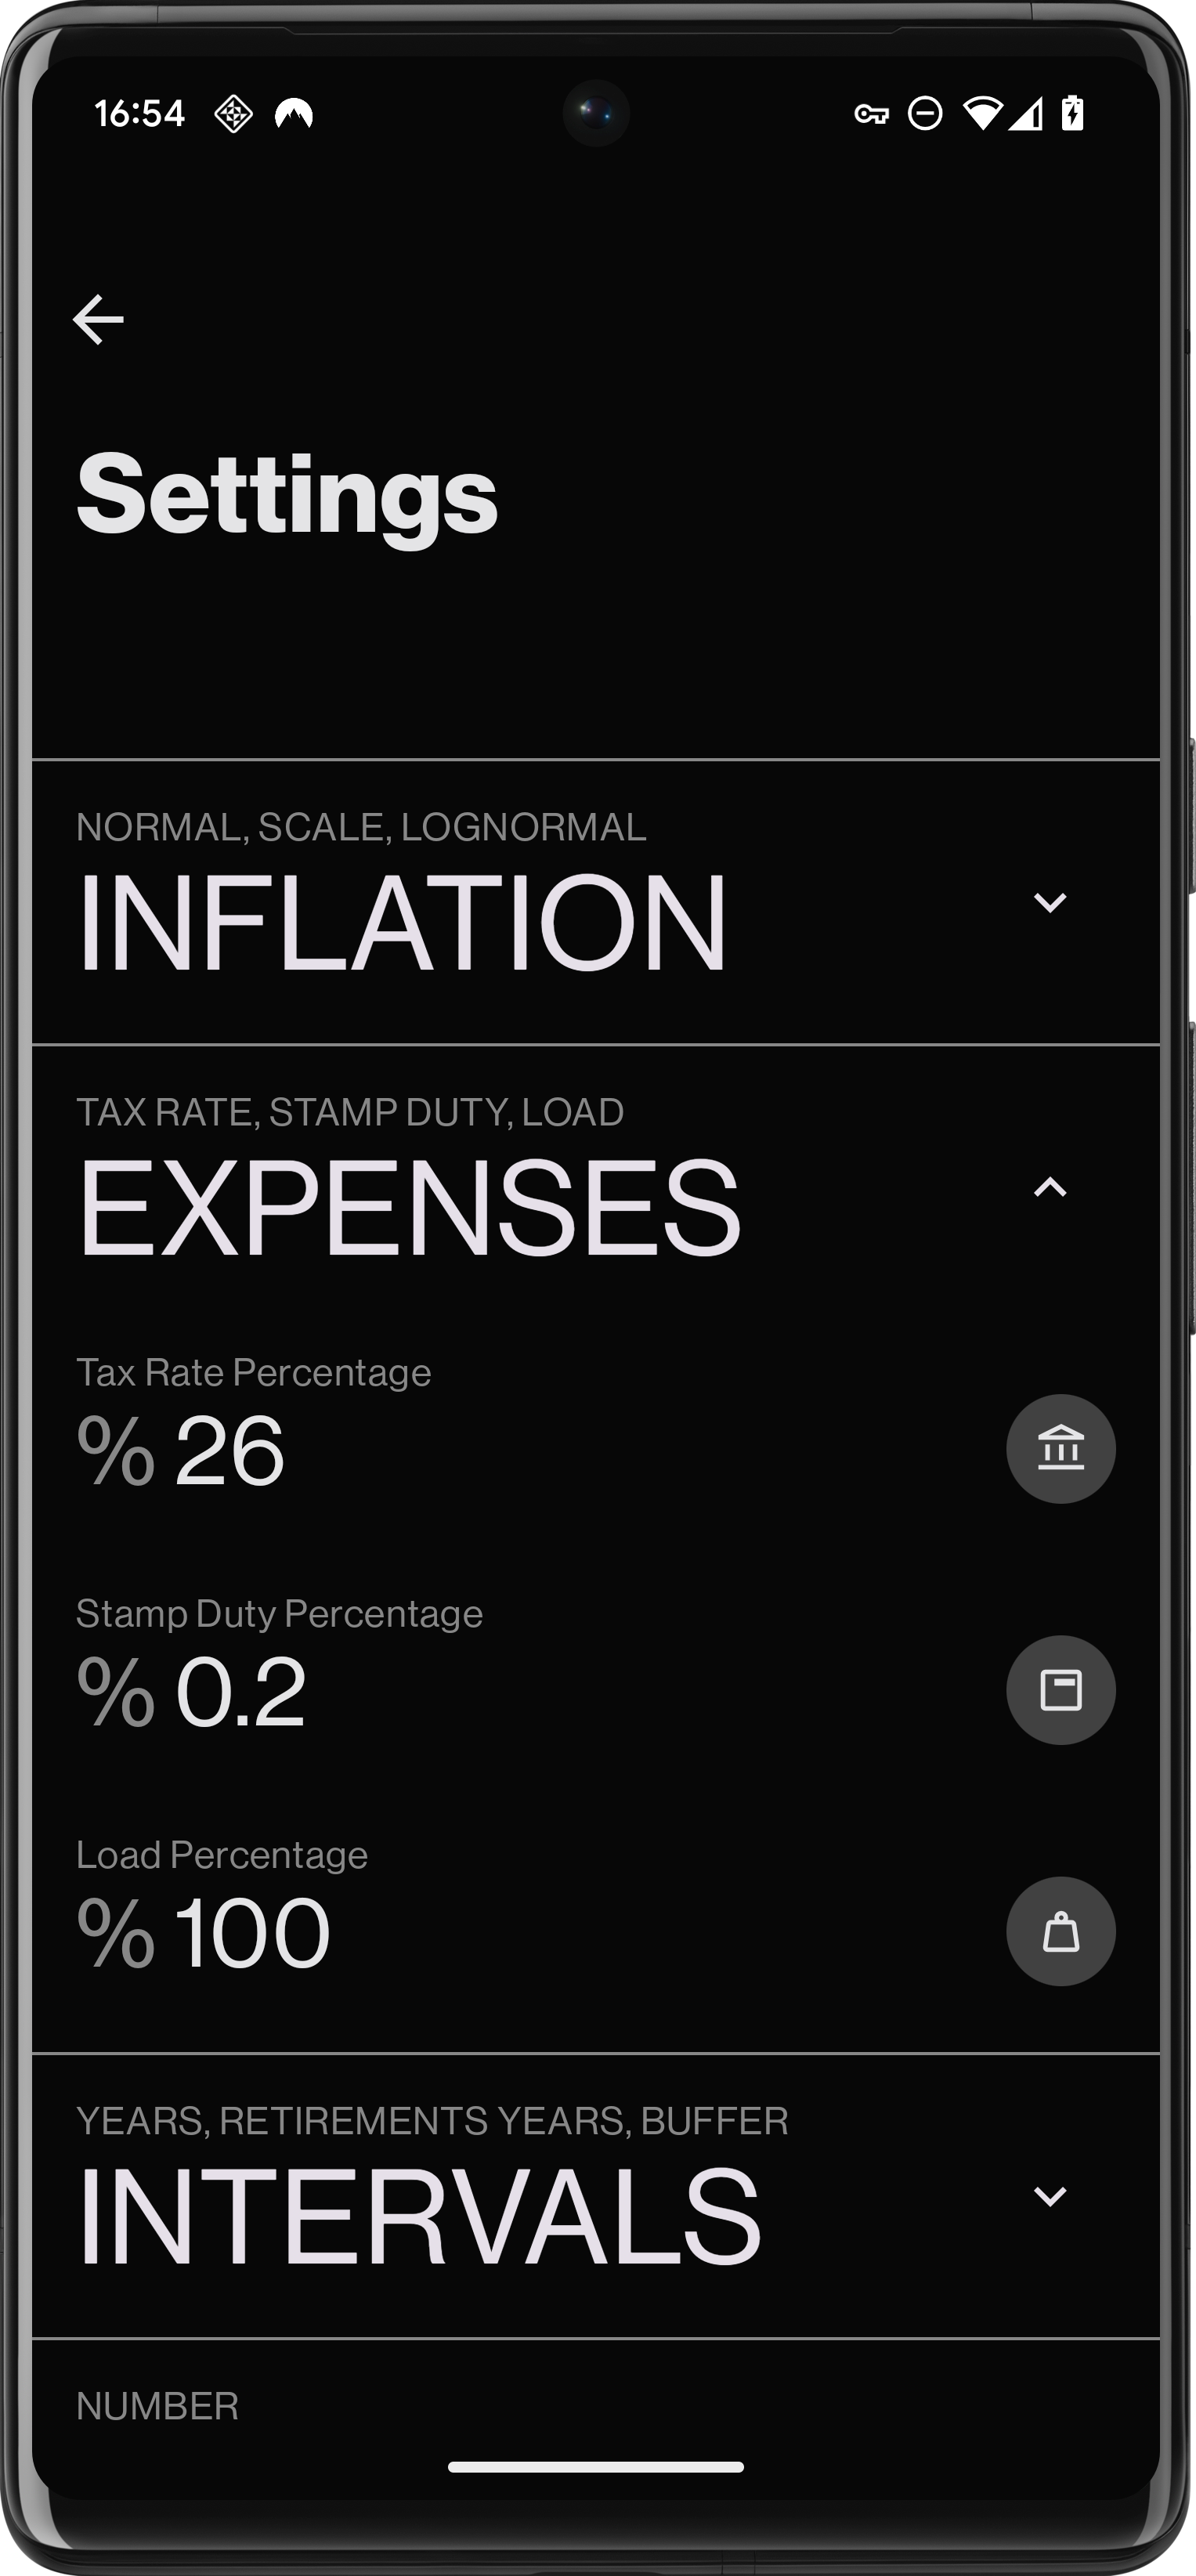
\includegraphics[width=\textwidth]{foto/input_card}
        \label{fig:input_card}
    \end{minipage}
\end{figure}